%% 
%% Copyright 2019 Elsevier Ltd
%% 
%% This file is part of the 'CAS Bundle'.
%% --------------------------------------
%% 
%% It may be distributed under the conditions of the LaTeX Project Public
%% License, either version 1.2 of this license or (at your option) any
%% later version.  The latest version of this license is in
%%    http://www.latex-project.org/lppl.txt
%% and version 1.2 or later is part of all distributions of LaTeX
%% version 1999/12/01 or later.
%% 
%% The list of all files belonging to the 'CAS Bundle' is
%% given in the file `manifest.txt'.
%% 
%% Template article for cas-dc documentclass for 
%% double column output.

% \documentclass[a4paper,fleqn,longmktitle]{cas-dc}
\documentclass[a4paper,fleqn]{cas-dc}

%\usepackage[authoryear,longnamesfirst]{natbib}
%\usepackage[authoryear]{natbib}
\usepackage[numbers]{natbib}
\usepackage{booktabs} % For formal tables
\usepackage{amsmath,amssymb,amsfonts,eucal}
% \usepackage{graphicx,subfigure}
\usepackage{algorithm,algorithmicx}
\usepackage{algpseudocode}
\usepackage{graphicx}
\usepackage{textcomp}
\usepackage{xcolor}
\usepackage{pifont}
\usepackage[misc]{ifsym}
\usepackage{multirow}
\usepackage{verbatim}
\usepackage{url}
\usepackage{soul}
\soulregister\cite7
\soulregister\ref7
% \usepackage[colorlinks, linkcolor=black, anchorcolor=red, citecolor=purple, urlcolor=blue]{hyperref}

\renewcommand{\algorithmicrequire}{\textbf{Input:}}
\renewcommand{\algorithmicensure}{\textbf{Output:}}


%%%Author definitions
\def\tsc#1{\csdef{#1}{\textsc{\lowercase{#1}}\xspace}}
\tsc{WGM}
\tsc{QE}
\tsc{EP}
\tsc{PMS}
\tsc{BEC}
\tsc{DE}
%%%

\begin{document}
\let\WriteBookmarks\relax
\def\floatpagepagefraction{1}
\def\textpagefraction{.001}
\shorttitle{P4DAD: Securing Duplicate Address Detection Using P4}
\shortauthors{Lin He et~al.}

\title [mode = title]{P4DAD: Securing Duplicate Address Detection Using P4}                      
% \tnotemark[1,2]

% \tnotetext[1]{This document is the results of the research
%    project funded by the National Science Foundation.}

% \tnotetext[2]{The second title footnote which is a longer text matter
%    to fill through the whole text width and overflow into
%    another line in the footnotes area of the first page.}


\author{Lin He}[orcid=0000-0002-7348-5833]
\author{Peng Kuang}
\author{Ying Liu}
\author{Gang Ren}
% \cormark[1]
\author{Jiahai Yang}
\address{Institute for Network Sciences and Cyberspace, Tsinghua University, Beijing 100084, China\\
Beijing National Research Center for Information Science and Technology (BNRist)
}

% \cortext[cor1]{Corresponding author.}

% \author[1,3]{CV Radhakrishnan}[type=editor,
%                         auid=000,bioid=1,
%                         prefix=Sir,
%                         role=Researcher,
%                         orcid=0000-0001-7511-2910]
% \cormark[1]
% \fnmark[1]
% \ead{cvr_1@tug.org.in}
% \ead[url]{www.cvr.cc, cvr@sayahna.org}

% \credit{Conceptualization of this study, Methodology, Software}

% \address[1]{Institute for Network Sciences and Cyberspace, Tsinghua University, Beijing 100084, China.}

% \author[2,4]{Han Theh Thanh}[style=chinese]

% \author[2,3]{CV Rajagopal}[%
%    role=Co-ordinator,
%    suffix=Jr,
%    ]
% \fnmark[2]
% \ead{cvr3@sayahna.org}
% \ead[URL]{www.sayahna.org}

% \credit{Data curation, Writing - Original draft preparation}

% \address[2]{Sayahna Foundation, Jagathy, Trivandrum 695014, India}

% \author%
% [1,3]
% {Rishi T.}
% \cormark[2]
% \fnmark[1,3]
% \ead{rishi@stmdocs.in}
% \ead[URL]{www.stmdocs.in}

% \address[3]{STM Document Engineering Pvt Ltd., Mepukada,
%     Malayinkil, Trivandrum 695571, India}

% \cortext[cor1]{Corresponding author}
% % \cortext[cor2]{Principal corresponding author}
% \fntext[fn1]{This is the first author footnote. but is common to third
%   author as well.}
% \fntext[fn2]{Another author footnote, this is a very long footnote and
%   it should be a really long footnote. But this footnote is not yet
%   sufficiently long enough to make two lines of footnote text.}

% \nonumnote{This note has no numbers. In this work we demonstrate $a_b$
%   the formation Y\_1 of a new type of polariton on the interface
%   between a cuprous oxide slab and a polystyrene micro-sphere placed
%   on the slab.
%   }

\begin{abstract}
    Duplicate Address Detection (DAD) is one of the functions of the Neighbor Discovery Protocol (NDP), which determines whether the IPv6 address of a node conflicts with those of other nodes. 
    However, due to the lack of verification of NDP messages, DAD is vulnerable to Denial of Service (DoS) attacks. 
    Existing solutions suffer from high complexity and low security, need to modify the NDP, or have a single point of failure, which renders them infeasible to be deployed.
     
    To solve the above problems, we propose P4DAD, which is a secure DAD mechanism based on P4. By creating and maintaining a binding entry between an IPv6 address and a link-layer property of a host's network attachment, P4DAD can filter spoofed NDP messages in an in-network manner to prevent DoS attacks on DAD without modification to the NDP or host stack. 
    We implement a prototype of P4DAD and evaluate it in terms of functionality, performance, and scalability. Evaluation results show that P4DAD can prevent DoS attacks on DAD successfully with negligible overhead and has satisfactory scalability.
\end{abstract}

% \begin{graphicalabstract}
% \includegraphics{grabs.pdf}
% \end{graphicalabstract} 

% \begin{highlights}
% \item Research highlights item 1
% \item Research highlights item 2
% \item Research highlights item 3
% \end{highlights}

\begin{keywords}
    Duplicate Address Detection \sep P4 \sep DoS attack \sep Neighbor Discovery Protocol \sep IPv6 
\end{keywords}

\maketitle

\section{Introduction}
    Duplicate Address Detection (DAD) is a crucial procedure in the process of IPv6 address configuration \cite{slaac}. It allows all nodes located on the same subnet to communicate and to join the network with unique IPv6 addresses. The DAD procedure is based on two Neighbor Discovery Protocol (NDP) \cite{NDP} messages, namely, Neighbor Solicitation (NS) and Neighbor Advertisement (NA).
    In DAD, a node sends one or more NS messages, and it will configure the target address only if no NA messages from existing nodes are received.
    Original DAD assumes that all nodes on a subnet are trustworthy. However, this assumption does not hold in the real network environment. 
    If a malicious node launches Denial of Service (DoS) attacks by replying to a victim's NS messages with spoofed NA messages continuously, the victim can not configure any IPv6 addresses.

    The above problem is severe due to its denial of a node's access to the network. 
    It will become more severe in the future because around 50 billion of the Internet of Things (IoT) devices will connect to the Internet by 2030 \cite{IOT3}. These IoT devices tend to use IPv6 addresses for communication  \cite{IoT-IPv6,LoWPAN}, and they still need to use DAD to determine the uniqueness of IPv6 addresses \cite{ipv6-iot}.
    
    To address this issue, many solutions have been proposed, which can be classified into three categories: target address hiding, NDP message authenticating, and uniform NA message replying. The first category is to use hash encryption or other mechanisms to hide target addresses in NS messages from unintended recipients. Malicious hosts cannot spoof NA messages effectively without knowing target addresses in NS messages.
    The second category is to append a message authentication code calculated by a hash function to each NDP message, which makes it possible for a host to distinguish valid messages from fake ones.
    The third category is to introduce a central node to reply with NA messages uniformly when receiving NS messages. Any NA messages sent by other nodes (including attackers) will be neglected.
    However, the first two solutions require the update of the NDP, which results in a large-scale modification to host network stack across different manufacturers and operating systems. The third solution always suffers a single point of failure, not to mention the lack of the design of address state update.
    
    In this paper, we ask the question: \emph{can we solve DoS attacks on DAD in an in-network manner without any modification to the existing standardized protocols or network architecture?} We are attracted to this solution because it neither requires modification to the host network stack nor introduces a central controller to change the communication mode.
    
    Recently, there has been a significant effort towards making network programmable, including data plane programming languages (e.g., P4 \cite{P4}) and the corresponding programmable targets (e.g., Barefoot Tofino \cite{tofino}), which enables unprecedented network flexibility, promising an ever-evolving set of network functionalities at hardware speeds \cite{yu2020netlock,zhang2020gallium,kim2020tea}.
    Inspired by this, we propose P4DAD, which can secure DAD in an in-network manner by leveraging P4.
    The core idea of P4DAD is to filter bogus NA messages of which the target addresses do not belong to the sender of NA messages. 
    
    P4DAD first uses P4 to monitor the address assignment procedure to create binding entries between an IPv6 address and a link-layer property of the host's network attachment (e.g., switch port). Then, P4DAD filters NA packets using binding entries to ensure the source address and target address of each NA packet are the same and belong to innocent hosts. P4DAD neither modifies the NDP nor requires a dependency on supportive functionality on hosts, which renders it widely deployable. 
    Moreover, as P4DAD does not introduce cryptographic encryption computation in the host and brings small processing overhead in the devices, it is lightweight. 
    Finally, P4DAD can be deployed on P4-enabled devices directly without the need for a central node, which makes it avoid single points of failure.

    In summary, the main contributions of this paper are as follows: 
    \begin{itemize}
        \item We conduct experiments on different operating systems and address assignment policies to show that DoS attacks on DAD are still very feasible and make hosts without network accessibility.

        \item We propose P4DAD, which is a lightweight, robust, and deployable DAD mechanism that can secure DAD in an in-network manner without any modification to the NDP or host network stack.

        % \item We propose a method allowing P4-enabled devices to configure and populate flow rules locally, avoiding the use of a remote central controller. 

        \item We implement a P4DAD prototype, and its evaluation results show that P4DAD can prevent DoS attacks on DAD in a lightweight, robust, and deployable manner.
    \end{itemize}
   
    The remainder of the paper is organized as follows: The related work is reviewed in Section \ref{sec:related work}. Section \ref{sec:threat model and design goals} describes the problem formulation of P4DAD. The details of P4DAD design are described in Section \ref{sec:p4dad design}. Section \ref{sec:implementation and evaluation} presents the implementation and evaluation of P4DAD. Security analysis is conducted in Section \ref{sec:security analysis}. The discussion is described in Section \ref{sec:discussion}. Finally, Section \ref{sec:conclusion} concludes the paper. 




\section{Related Work}\label{sec:related work}
    In this section, we start with a brief introduction of DoS attacks on DAD. Then, we present experimental results of how mainstream operating systems tackle DoS attacks on DAD as well as the influence of address assignment mechanisms on them. Next, we compare existing solutions and analyze their limitations. Finally, we give a brief introduction of P4 and explain why P4 is used for securing DAD.

    \subsection{DoS Attacks on DAD}
        DAD is used by a node to determine whether or not an address it wishes to use is already in use by another node.
        DAD must be performed on all unicast addresses before assigning them to an interface, regardless of whether they are obtained through manual configuration, Stateless Address Autoconfiguration (SLAAC) \cite{slaac}, or Dynamic Host Configuration Protocol for IPv6 (DHCPv6) \cite{DHCPv6}.
        As shown in Table \ref{tab:DAD}, in DAD, the source address of an NS message is unspecified; the destination address is a solicited-node multicast address where the NS message will be multicast; the target address in an NS message is the tentative address which a node (A) wants to configure.
        When the target address in the NS message is a duplicate, another node (B) with this address will reply with an NA message. Different from the NS message, the source address in the NA message is the interface address of B; the destination address is an all-node multicast address, which means the NA message will be multicast to all nodes on the same link\footnote{In this paper, the term ``link'' refers to a topological area bounded by routers that decrement the IPv4 TTL or IPv6 Hop Limit when forwarding the packet, which is the same as the definition in RFC 4903\cite{rfc4903}.}; the target address in the NA message is the IPv6 address on which A performs duplicate detection.
        
        \begin{table*}
            \centering
            \caption{Comparison of NS and NA messages in DAD.}
            \begin{tabular}{|c||c|c|c|}
                \hline
                \textbf{Message} & \textbf{Source Address} & \textbf{Destination Address} & \textbf{Target Address} \\
                \hline
                \hline
                NS & Unspecified & Solicited-node multicast address & Tentative address \\
                \hline
                NA & Interface address & All-node multicast address & Interface address \\
                \hline
            \end{tabular}
            \label{tab:DAD}
        \end{table*}

        During the procedure of DAD, a host first multicasts NS messages to verify the uniqueness of an IPv6 address, which it tries to configure. Generally, another host will reply with an NA message when it discovers the IPv6 address is a duplicate. However, it is easy for a malicious host to spoof NA messages because there exist no secure mechanisms to verify whether the sender of an NA message owns the IPv6 address or not. For example, Figure \ref{fig:DoS-Attack-on-DAD} sheds light on a DoS attack on DAD. When host C wants to configure a global unicast address $\mathtt{IP}_1$ (e.g., 2402::cf4e:3c0a:8490:88e1), it first multicasts an NS message to the link to verify the uniqueness of $\mathtt{IP}_1$. However, the attacker on the same link can reply with a spoofed NA message to indicate that $\mathtt{IP}_1$ is already used by another node. When host C tries to configure another address $\mathtt{IP}_2$ (e.g., 2402::f0f6:9824:f8e4:8900) and sends another NS message to verify the uniqueness of $\mathtt{IP}_2$, the attacker can also launch the attack by sending another NA message to indicate $\mathtt{IP}_2$ is already used. The result is that host C cannot configure any IPv6 addresses to its interfaces.

        \begin{figure}
        \centerline{
            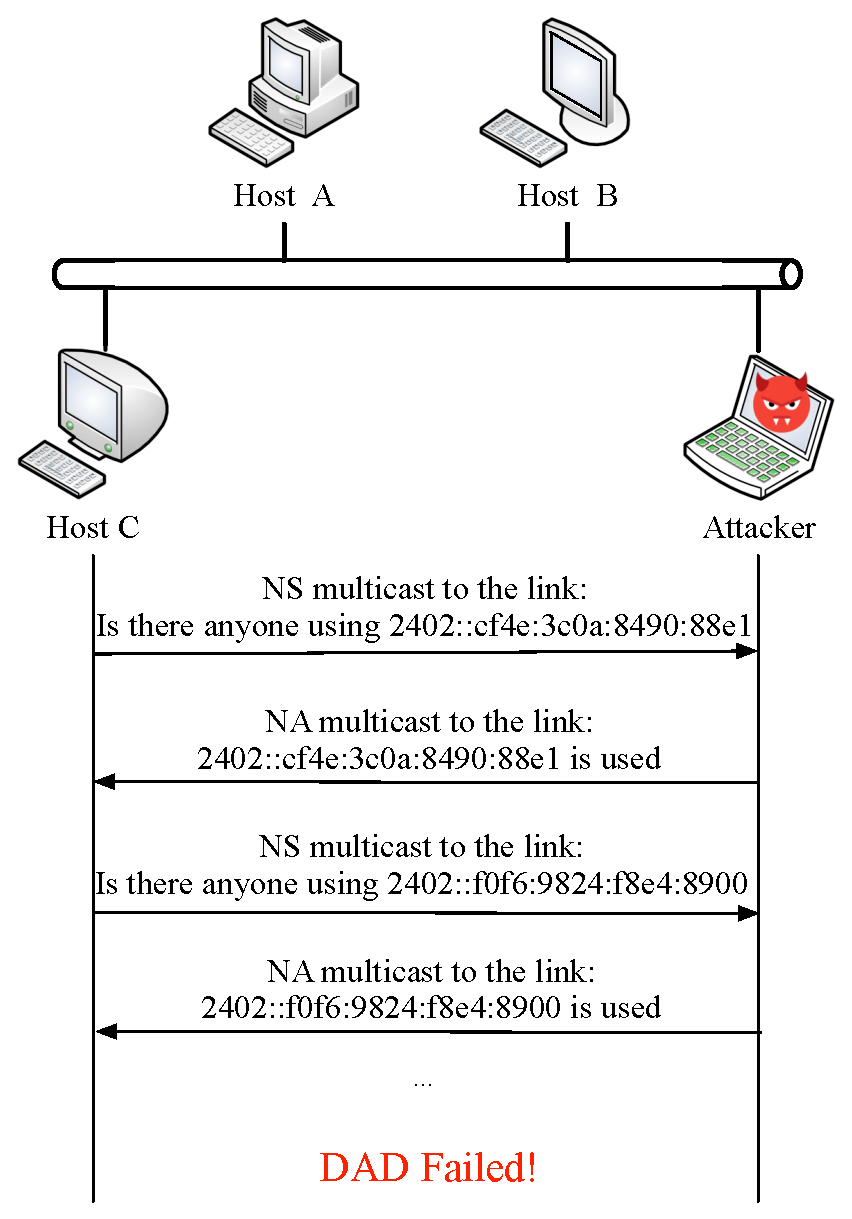
\includegraphics[scale=0.50]{figure/DAD-DoS.eps}
        }
        \caption{A DoS attack on DAD. Host C cannot configure any addresses to its interfaces when an attacker launches DoS attacks on DAD.}
        \label{fig:DoS-Attack-on-DAD}
        \end{figure}

        \begin{table*}
                \centering
                \caption{Test results of spoofed target addresses on link-local address autoconfiguration.}
                \begin{tabular}{|c||c|c|}
                    \hline
                    \textbf{Operating System} & 
                    \textbf{Source Address $=$ Target Address} & 
                    \textbf{Source Address $\neq$ Target Address} \\
                    \hline
                    \hline
                    Ubuntu 16.04 & Three tentative link-local addresses & Three tentative link-local addresses \\
                    \hline
                    CentOS 7.6 & Three DAD-failed link-local addresses & Three DAD-failed link-local addresses \\
                    \hline
                    Windows 10 & No link-local addresses & No link-local addresses \\
                    \hline
                    Windows 7 & No link-local addresses & No link-local addresses \\
                    \hline
                    macOS 10.15 & No link-local addresses & No link-local addresses \\
                    \hline
                \end{tabular}
                \label{tab:subnetLocal}
            \end{table*}

            \begin{table*}
                \centering
                \caption{Test results of spoofed NA messages in different address assignment mechanisms.}
                \begin{tabular}{|c||c|c|}
                    \hline
                    \textbf{Address Assignment Mechanism} & \textbf{Source Address $=$ Target Address} & \textbf{Source Address $\neq$ Target Address} \\
                    \hline
                    \hline
                    SLAAC & No global unicast addresses & No global unicast addresses \\
                    \hline
                    DHCPv6 & No global unicast addresses & No global unicast addresses \\
                    \hline
                    Manual Configuration & No global unicast addresses & No global unicast addresses \\
                    \hline
                \end{tabular}
                \label{tab:AddressAllocation}
            \end{table*}
    
    \subsection{Target Address Spoofing}
        We conduct two experiments on different operating systems and address assignment mechanisms to evaluate whether they influence the detection results of DAD when target addresses are spoofed in NA messages.

        \begin{itemize}
            \item \textbf{Different Operating Systems:}
            We build a simple topology where two hosts (a victim and an attacker) are connected to a switch. The victim sends an NS message to verify the uniqueness of a link-local address. At the same time, the attacker will reply with a spoofed NA message when receiving the NS message. We test two cases: 1) when the source address in the NA message is the same as the target address, and 2) when the source address in the NA message is different from the target address.
            The results are shown in Table \ref{tab:subnetLocal}. As we can see, the victim can not configure any link-local addresses successfully no matter whether the source address is equal to the target address or not on different operating systems. 

            \item \textbf{Different Address Assignment Mechanisms:}
            We also explore the influence of different address assignment mechanisms on the possibility of the attacker's launching DoS attacks on DAD when the target address is spoofed. Similarly, we also test two cases: 1) when the source address equals the target address in the NA message, 2) when the source address is not equal to the target address in the NA message.
            The results are shown in Table \ref{tab:AddressAllocation}. The victim can not configure any global addresses successfully regardless of whether they are obtained through SLAAC, DHCPv6, or manual configuration when the target addresses in NA messages are spoofed.
        \end{itemize}

        To conclude, mainstream operating systems do not check and filter spoofed NA messages no matter whether the tentative addresses are obtained through SLAAC, DHCPv6, or manual configuration, even when the source address is not the same as the target address in an NA message. Therefore, the target address in an NA message is the decisive factor which affects the detection result of DAD.



    \subsection{Existing Solutions}
        Currently, existing solutions to preventing DoS attacks on DAD can be classified into three categories: 1) hiding target addresses, 2) authenticating NDP messages, and 3) replying with NA messages uniformly.

        \begin{itemize}
        \item\textbf{Hiding Target Addresses:}
            The core idea of this kind of solution is to hide target addresses in NS messages during the procedure of DAD. DAD-match \cite{DAD-match} and Pull Model \cite{pull-model} embed the hash value of the target address instead of putting it directly in an NS message. Other hosts compute the hash values of their addresses and compare the results with the value in the NS message to determine whether they need to reply with NA messages. Wang et al. \cite{part-dad} proposed a mechanism that a host masks a segment of the target address, and other hosts compare the unmasked part of the target address and reply with standard NA messages if the unmasked part of the target address is a duplicate. The host collects all NA messages to determine whether the address is unique or not. Although this kind of solution can mitigate DoS attacks on DAD, they require modification to the NDP and host stack, which makes it challenging to deploy in the current networks.
        %DAD-h\cite{song2016novel}

        \item\textbf{Authenticating NDP Messages:}
            This kind of solution enhances DAD security by appending a message authentication code to each NDP message. Trust-ND \cite{trust-nd} and Secure-DAD \cite{secure-dad} are representatives of the methods of this type, which calculate the message authentication code by using SHA-1 and UMAC hash function, respectively. 
            However, Trust-ND is not secure because it is vulnerable to collision attacks due to its design. Moreover, an attacker can also use SHA-1 to compute correct message authentication codes and append them to spoofed NA messages to launch DoS attacks on DAD. Secure-DAD does not address how secret keys are shared between a new host and existing hosts. If all the hosts share the same key, an attacker on the same link can also launch DoS attacks. If a new host is required to establish secret keys with all existing hosts, an attacker can still use the secret key shared with the new host to compute message authentication codes and launch DoS attacks, not to mention the scalability of key exchange between hosts.
            % By utilizing the characteristic that it is difficult for malicious hosts to forge the same message authentication code, benign hosts can distinguish valid messages from spoofed ones. 
            Besides, they both introduce new options to NDP messages, which also requires modification to the NDP and host stack. 
        
        \item\textbf{Replying with NA Messages Uniformly:}
            The last kind of solution is to utilize a central reliable node to reply with NA messages uniformly, and any other NA messages sent by other nodes will be neglected. Nelle et al. \cite{ndp-proxy} used a Software-Defined Networking (SDN) switch as an NDP proxy that intercepts all NDP messages and forwards them to the SDN controller. As the controller stores all the assigned IPv6 addresses, it replies an NA message if a tentative address is a duplicate. Rule-based mechanism \cite{Controller-Scheme} uses a central node to store all configured IPv6 addresses. Other nodes must receive its confirmation messages to verify whether a tentative address is a duplicate or not. However, SDN suffers from a lot of security issues \cite{DBLP:conf/sdn4fns/Scott-HaywardOS13,DBLP:journals/comsur/Scott-HaywardNS16,DBLP:journals/comsur/AhmadNYG15}, e.g., DoS attacks. Both of them need a central node to store all IPv6 addresses, which thus becomes a single point of failure and renders the whole network down in case of a security compromise. Moreover, Rule-based mechanism also requires modification to the NDP.
        \end{itemize}

        Table \ref{tab:mechanism-feature} summarizes the comparison and limitations of existing solutions. We aim to design P4DAD to overcome these limitations.
            
            \begin{table*}
                \centering
                \caption{Comparison of existing solutions.}
                \small
                \begin{tabular}{|r||r||c|c|c|c|}
                    \hline
                    \textbf{Type} & \textbf{Mechanism} & \textbf{Secure} & \textbf{Lightweight} & \textbf{Robust} & \textbf{Deployable} \\
                    \hline
                    \hline
                    \multirow{3}{*}{Hiding Target Addresses} & DAD-match \cite{DAD-match} & \ding{51} &   & \ding{51} &  \\
                    \cline{2-6}
                    &Pull Model \cite{pull-model} & \ding{51} &   & \ding{51} &  \\
                    \cline{2-6}
                    &Wang et al. \cite{part-dad} & \ding{51} &   & \ding{51} &  \\
                    \hline
                    \hline
                    % DAD-h & \ding{51} &  & \ding{51} \\

                    \multirow{2}{*}{Authenticating NDP messages} & Secure-DAD \cite{secure-dad} &  &   & \ding{51} &  \\
                    \cline{2-6}
                    &Trust-ND \cite{trust-nd} &  &   & \ding{51} &  \\
                    \hline
                    \hline

                    \multirow{2}{*}{Replying with NA Messages Uniformly} & Nelle et al. \cite{ndp-proxy} &  & \ding{51} &  & \ding{51}\\
                    \cline{2-6}
                    &Rule-based \cite{Controller-Scheme} & \ding{51} & \ding{51} & &  \\
                    \hline
                    \hline

                    \textbf{Monitoring \& Filtering} & \textbf{P4DAD} & \ding{51} & \ding{51} & \ding{51} & \ding{51} \\
                    \hline
                \end{tabular}
                \label{tab:mechanism-feature}
            \end{table*}


    \subsection{Programmable Devices and P4}
        % \hl{
        P4 \cite{P4} is a domain-specific language for programming switching ASICs (Application-Specific Integrated Circuits) based on the reconfigurable match tables (RMT) model \cite{RMT}.
        As shown in Figure \ref{fig:P4Switch}, RMT consists of five components, i.e., the parser, ingress pipeline, queue, egress pipeline, and deparser.
        The parser is used to extract user-defined header fields.
        The ingress and egress pipelines contain a sequence of logical match-action stages, which can match specific header fields and perform corresponding actions. The queuing system between ingress and egress pipeline is associated with common data buffers to store packets. The deparser is used to reconstruct a packet after the egress pipeline.
        Moreover, P4 supports stateful components, e.g., registers, counters, to store states in the data plane directly.
        A P4 program only defines data plane functions and requires flow rules from the control plane to decide which action to take for each packet.
        
        Given the flexibility, we briefly highlight the new opportunities that programmable devices bring for preventing DoS attacks on DAD. In the DAD scenario, the programmable parser in P4 can be defined to extract target addresses in NS and NA messages. Besides, P4 can utilize stateful registers to preserve binding entries in the data plane directly. Therefore, P4DAD can monitor DAD procedures to create binding entries between legal addresses of each host and switch port, and then use them to filter spoofed NS and NA messages.
        
        Compared with the previous version of this paper \cite{DBLP:conf/icc/KuangLH20}, we have made substantive enhancements in this manuscript.
        Firstly, we conduct experiments to prove that mainstream operating systems do not check and filter spoofed NA messages no matter how the tentative addresses are obtained, which indicates an attacker can launch DoS attacks on DAD easily.
        Secondly, we have thoroughly optimized the binding entry update algorithm (including the design of binding entry expiration mechanism) and provided the target address validation algorithm for P4DAD.
        Finally, we have updated the evaluation and discussed the deployment strategies of P4DAD to demonstrate that P4DAD can enhance DAD security in a lightweight, robust, and deployable manner.
        % }
        \begin{figure}
                \centerline{
                    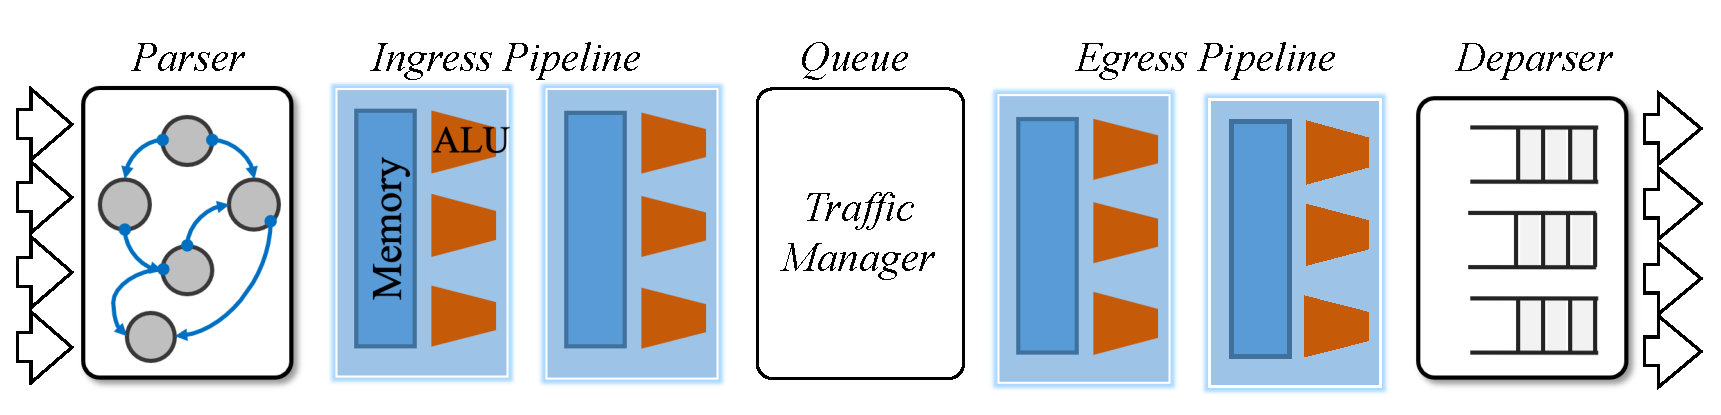
\includegraphics[scale=0.3]{figure/RMT.eps}
                }
                \caption{Switch chip architecture.}
                \label{fig:P4Switch}
        \end{figure} 


\section{Problem Formulation}\label{sec:threat model and design goals}
    \subsection{Design goals}
        P4DAD aims to enhance DAD security without introducing any modification to the NDP and host stack in a lightweight and robust manner, which implies three goals:
        \begin{itemize}
            \item\textbf{Lightweight}: P4DAD should not introduce hash encryption computation to hosts or network devices, which will increase computation complexity. Besides, P4DAD should only bring a small performance overhead to switches.

            \item \textbf{Robust}: 
            P4DAD should not introduce a central node, which requires that P4DAD be able to prevent DoS attacks on DAD in a distributed manner, which ensures that P4DAD can avoid a single point of failure problem.

            \item \textbf{Deployable}: 
            P4DAD should not modify the NDP or host stack. It means P4DAD should be designed to be purely network-based, which enables network operators to deploy it without a dependency on supportive functionality on hosts. 
        \end{itemize}


    \subsection{Threat Model}\label{sec:threat model}
        We assume that hosts on a link connect to P4DAD-enabled devices (e.g., P4 switches) directly. We relax this assumption in Section \ref{sec:aggregation} and discuss the deployment strategy when first-hop devices do not upgrade to support P4DAD.
        % In IoT networks, a host is an IoT node, and a switch is an IoT gateway or IoT proxy \cite{ipv6-iot}.
        It is also assumed that hosts may be malicious and can send arbitrary spoofed NDP messages, which may contain spoofed source addresses or target addresses. Besides, we assume that P4DAD-enabled devices are trustworthy and can process received NDP messages correctly.
        
    \subsection{Challenges}
        To design P4DAD, we mainly face three challenges:
        \begin{enumerate}[1)]
            \item \textbf{Multiple IPv6 Addresses Per Host}: In IPv6 networks, a host usually configures more than one IPv6 address. One is a link-local address, and the others may be assigned by SLAAC, DHCPv6, or manual configuration. How to deal with them in P4DAD is challenging.
            
            \item \textbf{Auto-Configuration of Flow Rules without a Central Controller}: P4 is a data plane programming language that can be used to describe how to parse and handle packets. P4 programs often use flow rules from the control plane to decide which action to take for every packet. Although P4Runtime \cite{p4runtime} provides a control plane programming interface to configure and populate flow rules, it needs to maintain complete network topology information, which may be a single point of failure. How to configure and populate flow rules in switches locally is a challenge.

            \item \textbf{Address State Change without Timer}: During the procedure of P4DAD, there are two updates of the address state. Firstly, when a binding entry is established, P4DAD will set the state of an IPv6 address as ``tentative''. If there are no NA messages received within a certain period of time (e.g., 1 second \cite{slaac}), the address will pass the DAD procedure, and its state will be updated as ``preferred''. 
            Secondly, each preferred address has a lifetime. For example, in DHCPv6, the preferred lifetime will be carried in Reply messages \cite{DHCPv6} when assigning an IPv6 address to a client. In SLAAC, the preferred lifetime will be carried in the Prefix Information option in Router Advertisement messages. A preferred address becomes deprecated when its preferred lifetime expires. 
            P4DAD should update or clear the expired binding entries in time. However, in the current version of P4 \cite{P4}, there is no related timer mechanism. Thus, how to change the address state without a timer is a challenge.
        \end{enumerate}



\section{P4DAD Design}\label{sec:p4dad design}
    This section presents the details of P4DAD design. Generally, P4DAD utilizes two key features of P4 to secure DAD:
    \begin{itemize}
        \item it uses the programmable parser to extract target addresses in NS and NA messages;
        \item it uses stateful memory registers to preserve bindings between link-layer properties of nodes' network attachment (e.g., ports) and IPv6 addresses in the data plane directly.
    \end{itemize}

    To solve the problem of multiple IPv6 addresses assigned to a single host, P4DAD allows a switch port\footnote{We take P4 switches as an example to demonstrate the design of P4DAD. In wired networks, we use switch ports to create bindings. In wireless networks, we can create bindings between MAC addresses and IPv6 addresses. The security of MAC address is assured by 802.11i or other mechanisms.} to correspond to multiple IPv6 addresses. To realize the auto-configuration of flow rules, P4DAD uploads the digest of required information in packets to the control plane and notifies it of populating appropriate flow rules in real-time. As for the address state change, we utilize a ``sketchy timer'' to solve it (See more details in Section \ref{sec:binding-entry-update}).

    \subsection{Overview of P4DAD}
        On the whole, P4DAD is composed of a data plane and a control plane. As shown in Figure \ref{fig:P4DAD-Overview}, the data plane contains a parser, pipeline, deparser, and registers. The parser is responsible for extracting the header of each NS or NA message for processing by pipeline. The pipeline is the core component of the data plane composed of if-else structures and match-action tables (MATs). As shown in Table \ref{tab:NS-NA-Function}, the pipeline performs different operations on NS and NA messages for different functions. First, the pipeline verifies the source and target addresses in the header to drop spoofed packets (Section \ref{sec:source and target validation}). Then, it sends MAC addresses and ingress ports to the control plane for MAC address learning (Section \ref{sec:self-learning building}). Next, it queries the target address to determine whether to update the binding entry of IPv6 address and port in the register (Section \ref{sec:binding-entry-update}). Finally, it forwards packets based on destination MAC addresses.
        The control plane is a local controller of the switch, which receives information from the data plane and populates appropriate flow rules promptly.

        \begin{figure*}
        \centerline{
            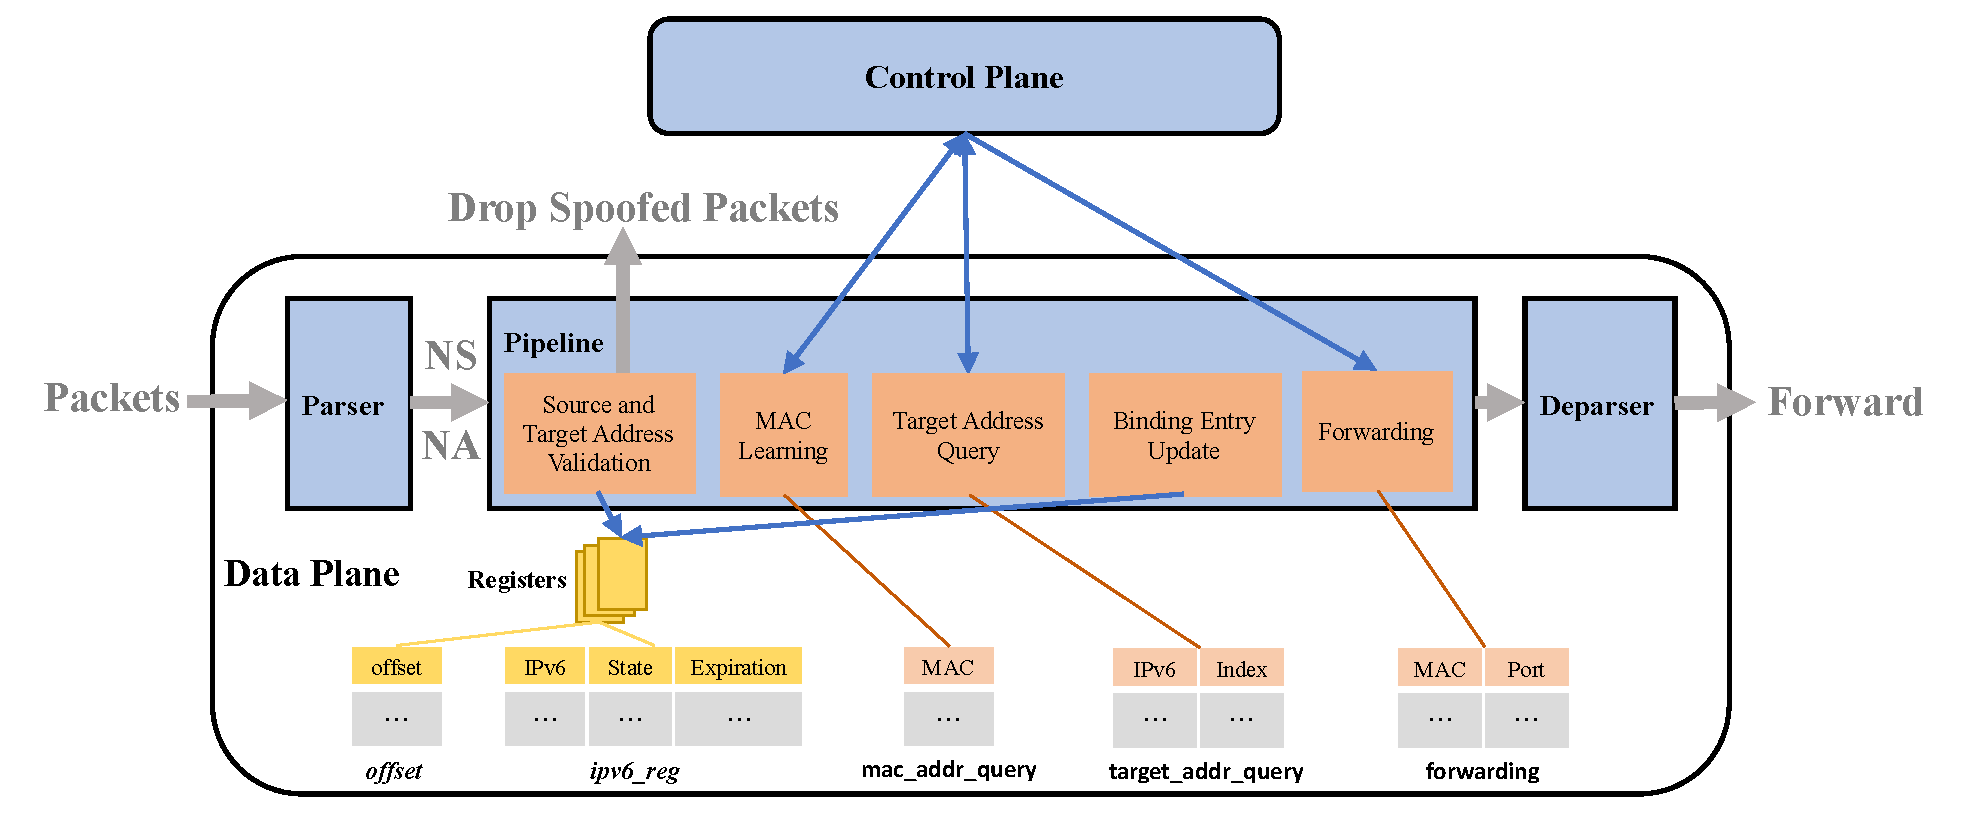
\includegraphics[scale=0.5]{figure/Overview.eps}
        }
        \caption{Design overview of P4DAD.}
        \label{fig:P4DAD-Overview}
        \end{figure*}

        \begin{table*}
            \centering
            \caption{Different operations on NS and NA messages for different functions.}
            % \begin{tabular}{llllllll}
            \begin{tabular}{|m{1.1cm}<{\centering}||c|m{1.6cm}<{\centering}|m{1.6cm}<{\centering}|m{1.4cm}<{\centering}|m{1cm}<{\centering}|m{1.9cm}<{\centering}|c|}
                \hline
                \textbf{Message Type} & \textbf{Function} & \textbf{Source Validation} & \textbf{Target Validation} & \textbf{MAC Learning} & \textbf{Target Query} & \textbf{Binding Entry Update} & \textbf{Forwarding} \\
                \hline
                \hline
                \multirow{3}{*}{NS} & DAD &  &  & \ding{51} & \ding{51} & \ding{51} & \ding{51} \\
                \cline{2-8}
                 & Address Resolution & \ding{51} &  &  &  &  & \ding{51} \\
                \cline{2-8}
                 & Unreachability Detection & \ding{51} &  &  &  &  & \ding{51} \\
                \hline
                \hline
                \multirow{4}{*}{NA} & DAD & \ding{51} & \ding{51} &  & \ding{51} & \ding{51} & \ding{51} \\
                \cline{2-8}
                 & Address Resolution & \ding{51} &  &  & \ding{51} &  & \ding{51} \\
                \cline{2-8}
                 & Unreachability Detection & \ding{51} &  &  & \ding{51} &  & \ding{51} \\
                \cline{2-8}
                 & Unsolicited & \ding{51} &  &  & \ding{51} &  & \ding{51} \\
                \hline
            \end{tabular}
            \label{tab:NS-NA-Function}
        \end{table*}

        \begin{figure*}
        \centerline{
            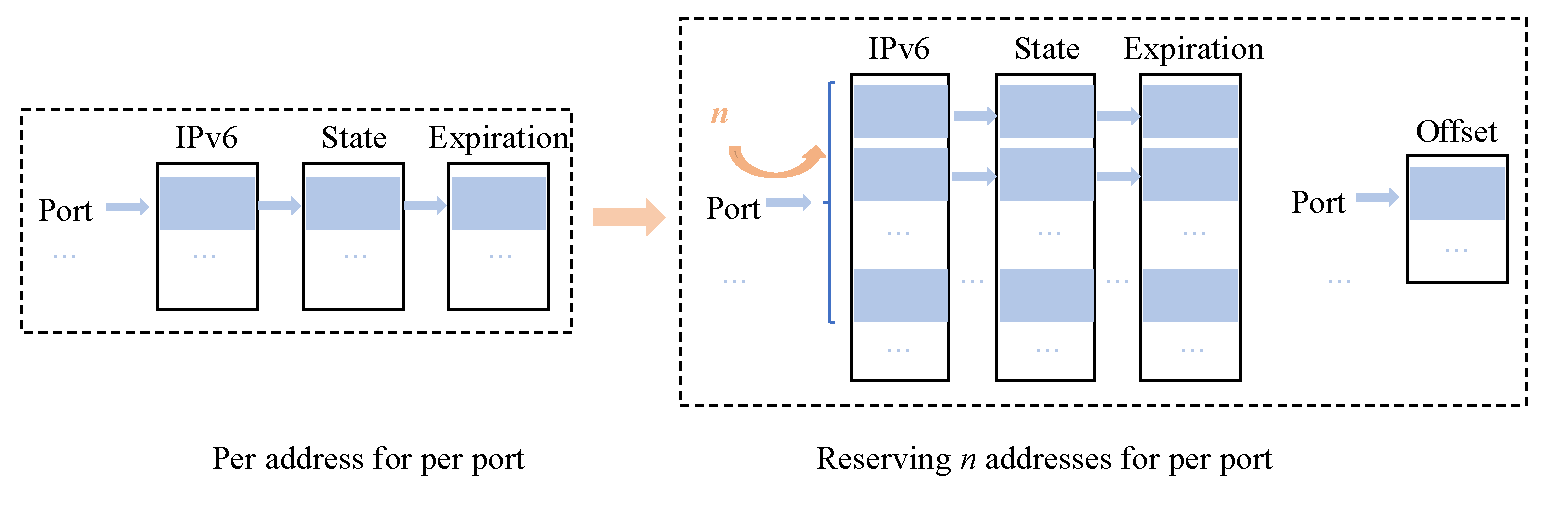
\includegraphics[scale=0.65]{figure/Register.eps}
        }
        \caption{Register design for P4DAD.}
        \label{fig:register}
        \end{figure*}


    \subsection{Source and Target Validation}\label{sec:source and target validation}
        To verify the authenticity of the source and target addresses in NS and NA messages, P4DAD utilizes bindings between IPv6 addresses and their corresponding switch ports. More details of creating and updating binding entries are provided in Section \ref{sec:binding-entry-update}. When a P4 switch receives a packet from a host, it first checks whether the packet is an NDP message. If the packet is an NS message, the switch first determines whether it is used for DAD. If the NS message is used for DAD, the switch just forwards the packet; otherwise, the switch queries the source address of the NS packet in $ipv6\_reg$ to determine whether to forward the packet.
        If the packet is an NA message, the switch first validates whether the source address equals the target address or not. Spoofed NA messages will be dropped. Then, it queries the target address in $ipv6\_reg$ to determine whether to forward the packet. If the above check fails, the switch drops the packet; otherwise, it forwards the packet.
        The above steps are summarized in Algorithm \ref{alg:validation}.

        \begin{algorithm}[!t]
        \caption{Source and Target Address Validation in P4DAD.}
        \label{alg:validation}
            \begin{algorithmic}[1]
            \Require $pkt$, $meta$, $ipv6\_reg$, $offset$, $n$\\
            $\triangleright$ $pkt$ refers to an ICMPv6 packet.\\
            $\triangleright$ $meta$ refers to the metadata associated with a packet, e.g., ingress port.\\
            % $\triangleright$ $\mathsf{target\_addr\_query}$ refers to a match-action table used to query target addresses\\
            $\triangleright$ $ipv6\_reg$ refers to a register used to store IPv6 addresses corresponding to each port.\\
            $\triangleright$ $of\!\!f\!set$ refers to a register used to store the offset corresponding to each port.\\
            $\triangleright$ $n$ refers to the maximum number of addresses that the register can store for each host.

            \State $ip_{src} \gets pkt[source\_address]$
            \State $ip_{dst} \gets pkt[destination\_address]$ 
            \If {$pkt$ is NS}
                \State $ip_{tgt} \gets pkt[target\_address]$
                \If {$ip_{src}$ is not unspecified $\|$ $ip_{dst}$ is not a solicited-node multicast address}
                    \State $addrs$\! = \!\Call{readAddrs}{$meta$, $\!o\!f\!\!f\!set$, $n$, $ipv6\_reg$}
                    \If {$ip_{src}$ is not in $addrs$}
                        \State drop $pkt$
                    \EndIf
                \EndIf
            \ElsIf {$pkt$ is NA}
                % \If {$ip_{dst}$ is an all-node multicast address}
                \State $ip_{tgt} \gets pkt[target\_address]$
                \If {$ip_{tgt} != ip_{src}$}
                    \State drop $pkt$
                \EndIf
                \State $addrs$\! = \!\Call{readAddrs}{$meta$, $\!o\!f\!\!f\!set$, $n$, $ipv6\_reg$}
                \If {$ip_{tgt}$ is not in $addrs$}
                    \State drop $pkt$
                \EndIf
                % \Else
                %     \State $addrs$\! = \!\Call{readAddrs}{$meta$, $\!o\!f\!\!f\!set$, $n$, $ipv6\_reg$}
                %     \If {$ip_{src}$ is not in $addrs$}
                %         \State drop $pkt$
                %     \EndIf
                % \EndIf
            \EndIf
            \State forward $pkt$

            \State
            \Function{readAddrs}{$meta$, $of\!\!f\!set$, $n$, $ipv6\_reg$}
                \State $port \gets meta[ingress\_port]$
                \State $os \gets o\!f\!\!f\!set[port]$
                \State $index \gets n \cdot port$
                \State Delete the expired entries corresponding to $port$ and move the subsequent entries forward
                \State Read $os$ addresses into $addrs$ from $index$ in $ipv6\_reg$\\
                \quad\ \  \Return $addrs$ 
            \EndFunction
            \end{algorithmic}
        \end{algorithm}

        \textbf{Register Design}: P4DAD employs on-switch registers to store the bindings. Then, a key question is how to determine the entry in a register corresponding to a specific switch port, i.e., the method of calculating the register index.  
        Intuitively, as a host is connected to a port in a switch, a simple solution is to regard a switch port as the register index and set the host's IPv6 address as the corresponding value. 
        However, the following issue is that a host often has multiple IPv6 addresses. Therefore, we have to reserve multiple IPv6 addresses for every switch port in registers. 
        It is assumed that a host has $n$ IPv6 addresses ($n \geq 2$)\footnote{Generally, one is a link-local address, and the others are global unicast addresses, which are configured through manual configuration, SLAAC, or DHCPv6. Moreover, it is common practice for most mainstream operating systems to configure two SLAAC addresses for hosts.}. As P4$_{16}$ \cite{P4-16} only supports multiplication by a power of two currently, $n$ must be a power of two.
        The register index based on the switch port can be calculated as follows: 
        \begin{equation}
                \label{index-calculation}
                \begin{aligned}
                    index = n \cdot port + of\!fset,
                \end{aligned}
        \end{equation}
        where $port$ is the switch port number and $of\!fset$ is the number of IPv6 addresses currently stored in the register corresponding to the port. 

        To distinguish different IPv6 address states (e.g., tentative, preferred) \cite{slaac}, registers also need to store the state of each IPv6 address. As DAD is performed on the same link, registers can store 64-bit IPv6 interface identifiers without the common prefix. Figure \ref{fig:register} sheds light on the design of two registers P4DAD uses. More specifically, one register is used to store the IPv6 addresses and their corresponding states, and the other is used to store the offset corresponding to each port.



    \subsection{Self-learning Table Building}\label{sec:self-learning building}
        To avoid using a remote central controller to configure and populate flow rules, P4DAD implements MAC address and IPv6 address self-learning in switches locally. 
        Specifically, P4DAD employs three MATs, i.e., $\mathsf{mac\_addr\_query}$, $\mathsf{target\_addr\_query}$, and $\mathsf{forwarding}$, to query MAC addresses, query target addresses, and forward packets, respectively.

        The key issue of self-learning is how to notify the control plane of populating specified flow rules. Fortunately, P4$_{16}$ provides two methods to solve this problem: packet cloning and packet digest. The former is used to copy the entire content of packets to the control plane. The latter is used to send the digest of some fields in the packet to the control plane.
        As we only need to inform the control plane of the source MAC address and ingress port queried from the $\mathsf{mac\_addr\_query}$ and $\mathsf{forwarding}$, and the IPv6 address and register index from the $\mathsf{target\_addr\_query}$, we prefer to use packet digest in P4DAD.


        \begin{algorithm}[!t]
        \caption{Binding Entry Update for P4DAD.}
        \label{alg:binding-entry-update}
            \begin{algorithmic}[1]
            \Require $pkt$, $meta$, $\mathsf{target\_addr\_query}$, $ipv6\_reg$, $of\!fset$, $n$, ``T'', ``P''\\
            $\triangleright$ $pkt$ refers to an ICMPv6 packet.\\
            $\triangleright$ $meta$ refers to the metadata associated with a packet, e.g., ingress port.\\
            $\triangleright$ $\mathsf{target\_addr\_query}$ refers to a match-action table used to query target addresses.\\
            $\triangleright$ $ipv6\_reg$ refers to a register used to store IPv6 addresses corresponding to each port.\\
            $\triangleright$ $of\!fset$ refers to a register used to store the offset corresponding to each port.\\
            $\triangleright$ $n$ refers to the maximum number of addresses that the register can store for each host.\\
            $\triangleright$ $L$ refers to the lifetime of a $preferred$ address.\\
            $\triangleright$ ``T'' and ``P'' refer to the $tentative$ and $preferred$ states of an address, respectively.
            % $\triangleright$ ``T'' refers to the $tentative$ state of an address whose uniqueness on a link is being verified, prior to its assignment to an interface.\\
            % $\triangleright$ ``P'' refers to the $preferred$ state of an address assigned to an interface whose use by upper-layer protocols is unrestricted.

            \State $ip_{src} \gets pkt[source\_address]$
            \State $ip_{dst} \gets pkt[destination\_address]$
            \State $port \gets meta[ingress\_port]$
            \If {$pkt$ is NS \&\& $pkt$ comes from a host-connected port}
                \State $ip_{tgt} \gets pkt[target\_address]$
                \State Get the current timestamp $cur\_time$
                \If {$ip_{src}$ is unspecified \&\& $ip_{dst}$ is a solicited-node multicast address}
                    \If {$ip_{tgt}$\ misses \ $\mathsf{target\_addr\_query}$}
                        \State Delete the expired entries corresponding to $port$ and move the subsequent entries forward
                        % \State $port \gets meta[ingress\_port]$
                        \State $index \gets n \cdot port + of\!fset[port]$
                        \State $ipv6\_reg[index] \gets ip_{tgt}$,``T'', $cur\_time + 1$
                        \State $\mathsf{target\_addr\_query}[ip_{tgt}] \gets index$
                        \State $offset[port] \gets offset[port] + 1$
                    \EndIf
                \Else
                    \State $index \gets \mathsf{target\_addr\_query}[ip_{tgt}]$
                    \State $ipv6$, $state, exp\_time \gets ipv6\_reg$[$index$]
                    \If {$state$ == ``T'' \&\& $exp\_time < cur\_time$}
                        \State $ipv6\_reg[index]\!\gets\!ip_{tgt}$,``P'', \!$exp\_time +\! L -\! 1$
                    \EndIf
                \EndIf
            \ElsIf {$pkt$ is NA}
                \If {$ip_{dst}$ is an all-node multicast address}
                    \State $ip_{tgt} \gets pkt[target\_address]$ 
                    \If {$ip_{tgt}$ hits $\mathsf{target\_addr\_query}$}
                        \State $index \gets \mathsf{target\_addr\_query}[ip_{tgt}]$
                        \State $ipv6$, $state, exp\_time \gets ipv6\_reg$[$index$]
                        \If {$state$ == ``T''}
                            \State reset $ipv6\_reg$[$index$]
                            % \State $adjust(ipv6\_reg, index, n \cdot ( port + 1))$
                            \State reset $\mathsf{target\_addr\_query}[ip_{tgt}]$
                            \State $offset[port] \gets offset[port] - 1$
                        \EndIf
                    \EndIf
                \EndIf
            \EndIf
            \end{algorithmic}
        \end{algorithm}

    \subsection{Binding Entry Update}\label{sec:binding-entry-update}
        P4DAD creates bindings between IPv6 addresses and ports by listening to the NS and NA messages exchanged in the procedure of DAD. For NS and NA messages, P4DAD adopts different processing logic, which is summarized in Algorithm \ref{alg:binding-entry-update}. In P4DAD, there are two states for each address, namely $tentative$ and $preferred$. The $tentative$ state of an address means its uniqueness on a link is being verified, prior to its assignment to an interface. The $preferred$ state of an address assigned to an interface means its use by upper-layer protocols is unrestricted.

        First, P4DAD extracts the source and destination addresses from a packet. Then, P4DAD determines whether the packet is an NDP message. If the packet is an NS message, P4DAD extracts the target address in the packet. If the NS message is used for DAD, P4DAD queries whether the target address is in the $\mathsf{target\_addr\_query}$ or not. If the query misses, P4DAD first deletes the expired entries corresponding to the ingress port and moves the subsequent entries forward. Then, it calculates the register index based on the ingress port as shown in Equation (\ref{index-calculation}), and wraps the IPv6 address, its $tentative$ state, and expiration time in the corresponding register, which implies this is a new DAD procedure. The reason that we set 1 second after the current time as the expiration time is because the $tentative$ state of an IPv6 address will be expired in 1 second no matter what the result of the DAD procedure is. If the address is a duplicate, this entry will be deleted; otherwise, P4DAD will change the state of the address to $preferred$. 1 second is a default value as specified by IETF in RFC 4861 \cite{NDP}.
        If the NS message is not used for DAD, P4DAD changes the expired $tentative$ state of the target address to the $preferred$ state. In this case, when P4DAD receives an NS message not used for DAD, this means that the host directly connected to the P4 device starts to discover other nodes' presence, which implies the address passed the DAD procedure. Note that we solve challenge 3) by using a ``sketchy timer''. When the tentative state of an address expires, P4DAD will change its state into preferred after receiving NS messages for other functions rather than DAD. Because a tentative address of a host passes the DAD procedure after 1 second, the host will send NS messages for address resolution and unreachability detection, which triggers the change of address state in P4DAD. Similarly, if the preferred state of an address expires, P4DAD will delete this entry when receiving NS messages for DAD or filtering spoofed NS or NA messages corresponding to the same port.

        If the packet is an NA message used for DAD, P4DAD extracts the target address from the packet and queries it in the $\mathsf{target\_addr\_query}$. If the query hits, P4DAD acquires the index from the hitting entry and obtains IPv6 address and its state from the $ipv6\_reg$ using the index. If the state of IPv6 address is tentative, P4DAD resets the corresponding entry in $ipv6\_reg$ and $\mathsf{target\_addr\_query}$. This means the IPv6 address is used by another node on the link. After that, the addresses corresponding to a port should be adjusted to take up continuous space in a register.



    \subsection{P4DAD Workflow}
        We illustrate the P4DAD workflow in a simple network topology, which contains two P4 switches $\mathsf{S_1}$ and $\mathsf{S_2}$, as shown in Figure \ref{fig:P4DAD-Workflow}. Host $\mathsf{H_1}$ and $\mathsf{H_2}$ configured IPv6 addresses $\mathsf{IP_1}$ and $\mathsf{IP_2}$, respectively. Note that $\mathsf{H_2}$ is a malicious host, and it will launch DoS attacks on DAD. So the binding entries of $\mathsf{IP_1}$ and $\mathsf{IP_2}$ have been established in $\mathsf{S_1}$.
        $\mathsf{H_3}$ and $\mathsf{H_4}$ are performing DAD on addresses they wish to configure, respectively. $\mathsf{H_3}$ tries to configure the same IPv6 address as that (i.e., $\mathsf{IP_1}$) of $\mathsf{H_1}$. $\mathsf{H_4}$ wishes to configure a new IPv6 address $\mathsf{IP_3}$ to its interface.
        When receiving NS packets sent by $\mathsf{H_3}$ and $\mathsf{H_4}$, $\mathsf{S_2}$ will establish the binding entries of $\mathsf{IP_1}$ and $\mathsf{IP_3}$ and set the corresponding states of $\mathsf{IP_1}$ and $\mathsf{IP_3}$ to "Tentative". $\mathsf{H_1}$ will reply with an NA packet with $\mathsf{IP_1}$ as the source and target addresses. However, the malicious $\mathsf{H_2}$ will send two spoofed NA packets with $\mathsf{IP_1}$ and $\mathsf{IP_3}$ as the target address, respectively. When spoofed NA packets are received by $\mathsf{S_1}$, they will be filtered directly, which means the DoS attacks on DAD are prevented effectively. When $\mathsf{S_2}$ receives the NA packet sent by $\mathsf{H_1}$, the binding entry of $\mathsf{IP_1}$ will be cleared. When no NA packets with $\mathsf{IP_3}$ as the target address are received by $\mathsf{S_2}$ at a certain time, the corresponding state of $\mathsf{IP_3}$ will be set to ``Preferred''.  
        \begin{figure*}
            \centerline{
                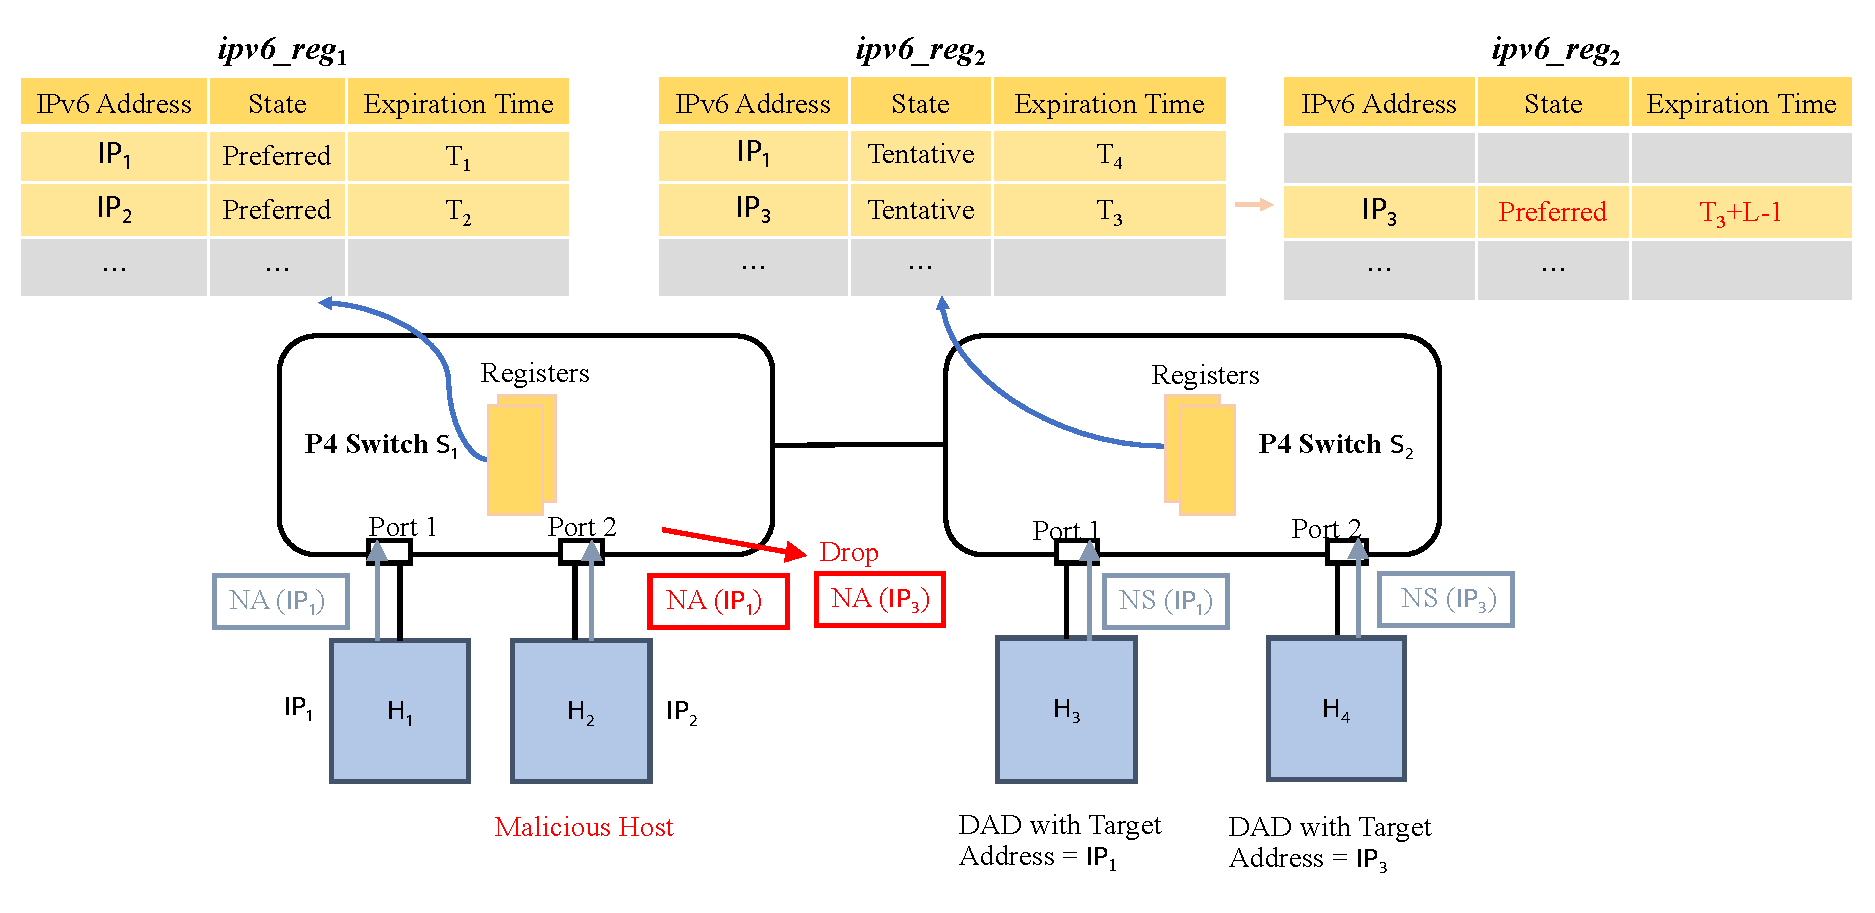
\includegraphics[scale=0.56]{figure/Workflow.eps}
            }
            \vspace{-0.3cm}
            \caption{An example of workflow for P4DAD.}
            \label{fig:P4DAD-Workflow}
            \vspace{-0.3cm}
        \end{figure*}


        % \subsection{\hl{Optimization}}





\section{Implementation and Evaluation}\label{sec:implementation and evaluation}
    In this section, we present the implementation and performance evaluation of P4DAD. 
    % First, we illustrate the P4DAD implementation.
    %Next, We measure host reactions when the source address is different from the target address in NA messages to verify whether the target address is the decisive factor which affects the detection results of DAD. 
    % Then, we evaluate the effectiveness of P4DAD on DoS attacks prevention. 
    % Next, we compare the processing time of NS/NA messages between P4DAD and baseline and measure the communication time between the data plane and the control plane to evaluate the performance of P4DAD.
    % Finally, we evaluate the scalability of P4DAD by measuring the P4 switch memory consumption when increasing the number of hosts.
    
    \subsection{Implementation}
        We implement a P4DAD prototype which is composed of a data plane program and a control plane program. The data plane program is implemented using P4$_{16}$ \cite{P4-16}, which can be compiled directly on bmv2 \cite{bmv2}. The control plane program is written in Python, which communicates with the data plane by notifications-addr \cite{bmv2}.

        Our experiments are conducted on a Dell OptiPlex 7050 server with Intel Core i7-7700 CPU (one core, 3.4 GHz) and 8 GB of memory.


    \subsection{Evaluation}
        % \hl{To evaluate the performance of P4DAD, we present several metrics:}
        % \begin{itemize}
        %     \item Message Processing Time:

        %     \item Digest Overhead:

        %     \item 
        % \end{itemize}

        \subsubsection{Functionality}
            We build a simple topology where 10 hosts (5 innocent hosts and 5 attackers) installed with the parasite6 tool are connected to a P4 software switch implemented by bmv2. 
            Both innocent hosts and attackers send NS and NA messages randomly. The difference is that innocent hosts send valid messages, while attackers send spoofed messages.
            % The attackers send spoofed NS or NA messages randomly.
            We count the number of packets received and filtered by P4DAD, sent by the attacker and the victim, respectively. The results are shown in Figure \ref{fig:P4DAD-filtered}. The number of NS and NA packets filtered by P4DAD is equal to that sent by the attacker, which means P4DAD can recognize and filter spoofed NS and NA messages effectively.
            \begin{figure}
                \centerline{
                    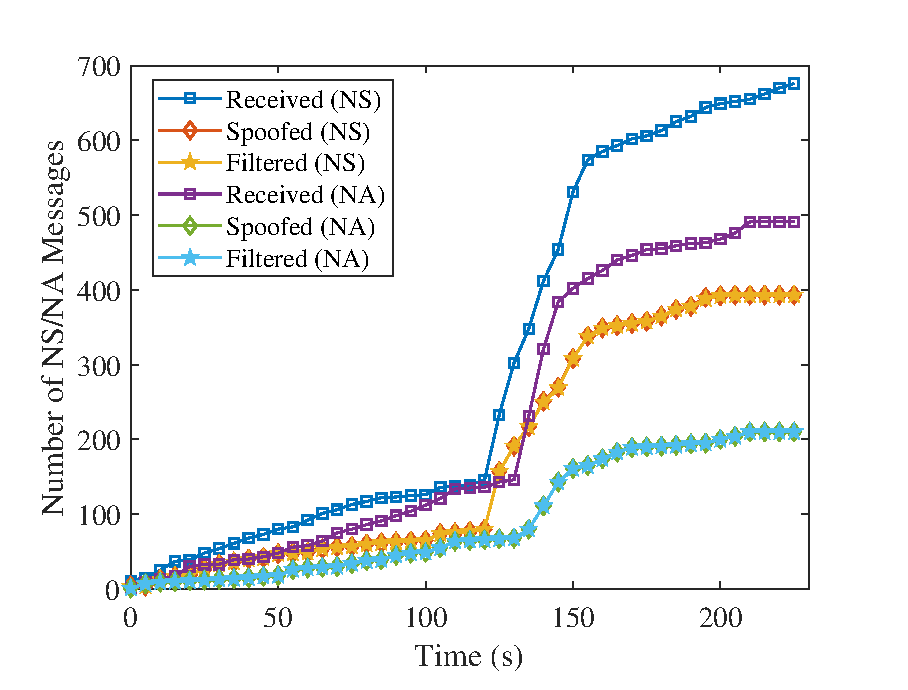
\includegraphics[scale=0.6]{figure/Filtered.eps}
                }
                \caption{Filtered messages using P4DAD.}
                \label{fig:P4DAD-filtered}
            \end{figure}


        \subsubsection{Performance}
            \textbf{Message Processing Overhead.} We use the performance of original NDP (no modification to switches) as the baseline and compare the processing time of NS and NA messages between P4DAD and the baseline. 
            As mentioned in Table \ref{tab:NS-NA-Function}, NS and NA messages have different usages in different scenarios. Therefore, for simplicity of notation, we denote NS-for-DAD and NS-for-Others as NS messages used to handle DAD and other NDP functions, respectively. Similarly, we denote NA-for-DAD and NA-for-Others as NA messages used to handle DAD and other NDP functions, respectively. As we expected, P4DAD increases processing time for each type of message by 27\%, 6.8\%, 36\%, and 14\% as shown in Figure \ref{fig:P4DAD-baseline}. This is because P4DAD introduces new operations and validates NDP messages to secure the security of DAD at the cost of slight performance degradation. More specifically, NA-for-DAD has the biggest increase in processing time because P4DAD utilizes several operations (i.e., source validation, target validation, target query, and binding entry update as shown in Table \ref{tab:NS-NA-Function}) to handle this type of messages. Conversely, NS-for-Others has the smallest increase in processing time because P4DAD only validates the source addresses for this type of message. In an IPv6 network, only when a host configures IPv6 addresses to its interfaces, NS-for-DAD and NA-for-DAD messages are used. Therefore, the message processing overhead introduced by P4DAD is lightweight.

            \textbf{Digest Overhead.} As the self-learning of P4DAD notifies the control plane of populating flow rules, we measure its overhead. Specifically, we measure the time from the beginning of the data plane's digesting packet information to the end of the control plane's populating flow rules. We conduct 1,000 tests, and its average time is 4.126 ms.
            Generally, the communication between the control plane and the data plane only occurs in the DAD procedure, and DAD only appears during the process of address configuration.
            % As mentioned above, NS-for-Others and NA-for-Others introduce much less overhead than NS-for-DAD and NA-for-DAD.
            Therefore, the processing overhead brought by packet digest is acceptable.

            % That is, most NS and NA messages are used for other NDP functions, e.g., address resolution, unreachability detection. As mentioned in Table \ref{tab:NS-NA-Function}, the processing time of NS and NA messages for other NDP functions  is much less than the baseline. Therefore, the processing overhead brought by P4DAD is negligible. } 
            
            \begin{figure}
            \centerline{
                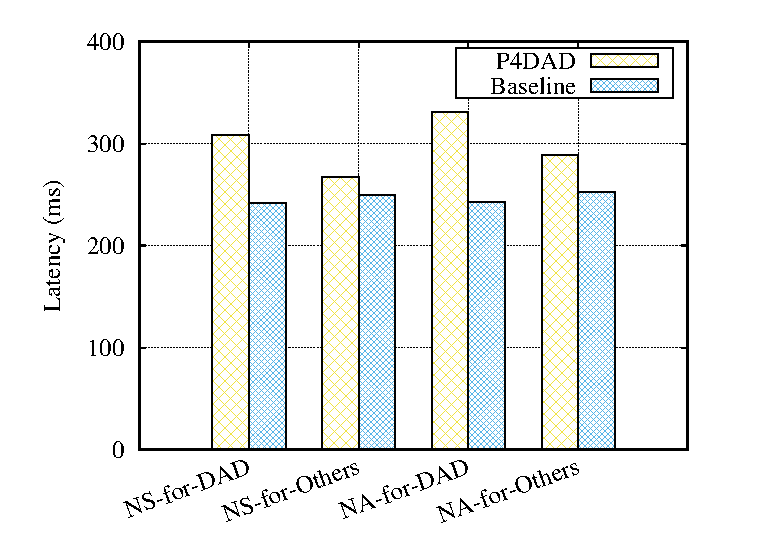
\includegraphics[scale=0.7]{figure/BaselineP4dad.eps}
            }
            \caption{Processing time of NS and NA messages in P4DAD.}
            \label{fig:P4DAD-baseline}
            \end{figure}

            % \begin{figure*}
            % \centering
            %     \begin{minipage}[t]{0.32\textwidth}
            %         \centering
            %         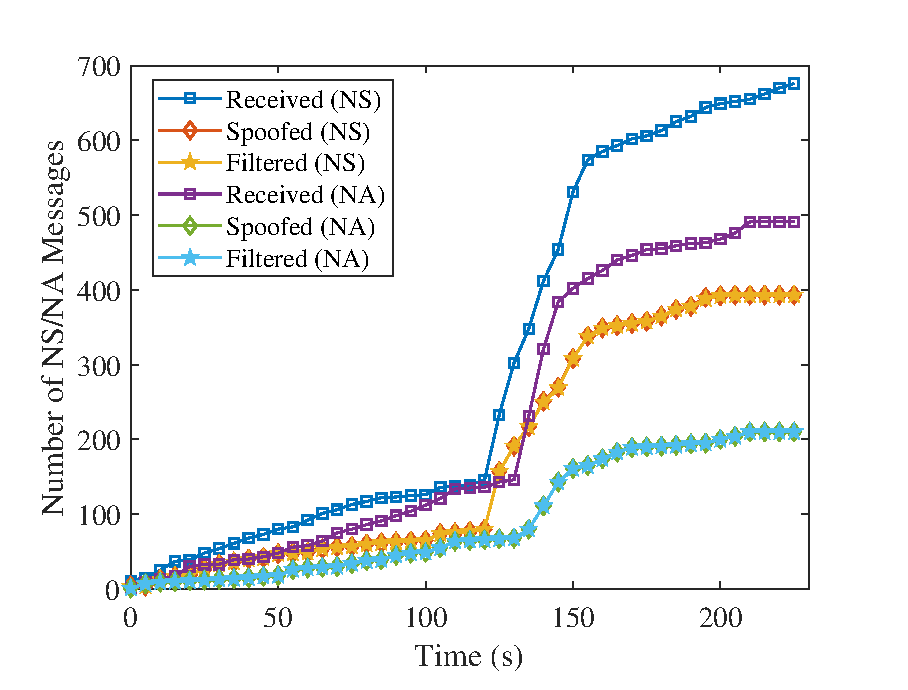
\includegraphics[width=6.5cm]{figure/Filtered.eps}
            %         \caption{Filtered messages using P4DAD.}
            %         \label{fig:P4DAD-filtered}
            %     \end{minipage}
            %     \begin{minipage}[t]{0.32\textwidth}
            %         \centering
            %         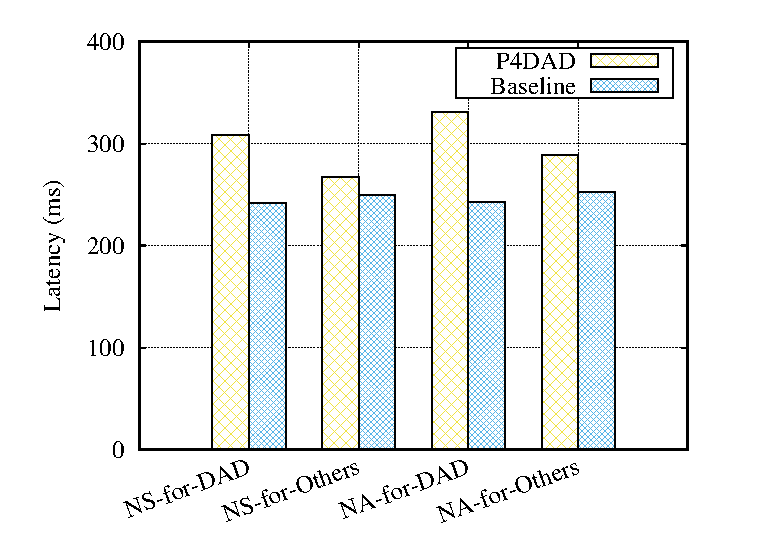
\includegraphics[width=6.5cm]{figure/BaselineP4dad.eps}
            %         \caption{Processing time of NS and NA messages in P4DAD.}
            %         \label{fig:P4DAD-baseline}
            %     \end{minipage}
            %     \begin{minipage}[t]{0.32\textwidth}
            %         \centering
            %         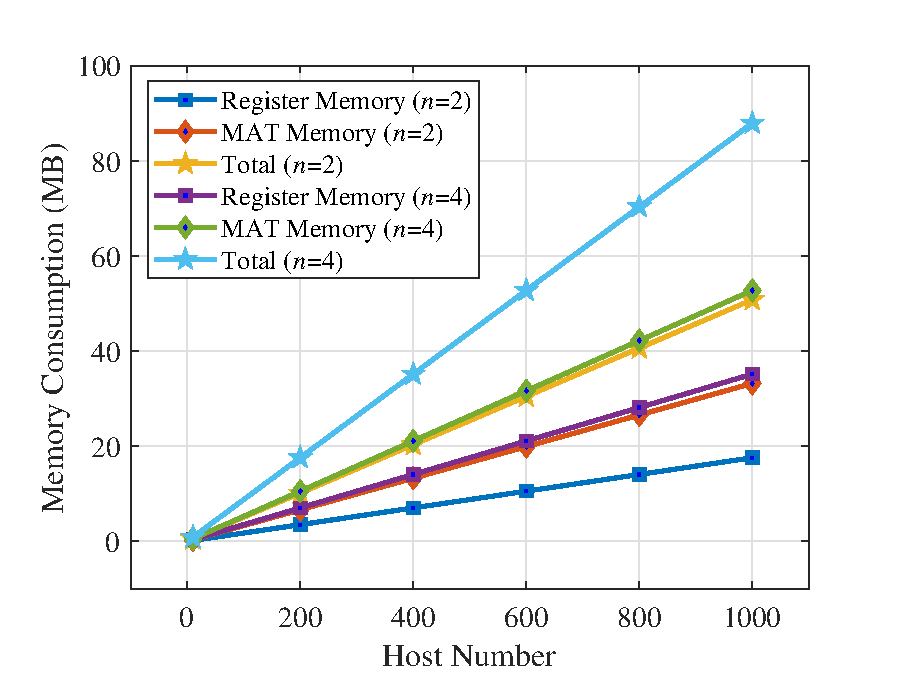
\includegraphics[width=6.5cm]{figure/MemoryConsumption.eps}
            %         \caption{Memory consumption of P4 switches.}
            %         \label{fig:Memory-Consumption}
            %     \end{minipage}
            % \end{figure*}

        \subsubsection{Scalability}\label{sec:scalability}
            In this paper, the scalability of P4DAD means the capability to cope and perform well when more and more hosts are connected to a P4 switch. More specifically, as the number of hosts connected to the P4 switch increases, the P4 switch will consume more memory to store the states of IPv6 addresses.
            % We measure the memory consumption of a P4 switch to evaluate the scalability of P4DAD when increasing the number of hosts. 
            The memory consumed by P4DAD consists of two folds: register memory and MAT memory. 
            We measure both of them and then calculate their sum.
            As shown in Figure \ref{fig:Memory-Consumption}, the memory consumption of P4DAD increases linearly with the number of hosts when $n$, as shown in Equation (\ref{index-calculation}), is equal to 2 or 4. When there are 1,000 hosts connected to P4 switches and $n=2$, $\sim$30 KB memory is consumed to store the states of IPv6 addresses, and $\sim$33 KB memory is used to store $\mathsf{mac\_addr\_query}$, $\mathsf{target\_addr\_query}$, and $\mathsf{forwarding}$.
            

            \begin{table*}
                \caption{Notation.}
                \centering
                \begin{tabular}{|r||l|}
                    \hline
                    \textbf{Symbol}&\textbf{Remarks}  \\
                    \hline
                    \hline
                    $b_i$  & Memory consumed by an IPv6 address\\
                    \hline
                    \specialrule{0em}{1pt}{1pt}
                    $b_s$  & Memory consumed by the state of an IPv6 address\\
                    \hline
                    \specialrule{0em}{1pt}{1pt}
                    $b_e$  & Memory consumed by expiration time of an IPv6 address\\
                    \hline
                    \specialrule{0em}{1pt}{1pt}
                    $b_o$  & Memory consumed by storing an offset in a register\\
                    \hline
                    \specialrule{0em}{1pt}{1pt}
                    $b_m$  & Memory consumed by storing a MAC address\\
                    \hline
                    \specialrule{0em}{1pt}{1pt}
                    $b_x$  & Memory consumed by storing the index of an IPv6 address in $\mathsf{target\_addr\_query}$\\
                    \hline
                    \specialrule{0em}{1pt}{1pt}
                    $b_p$  & Memory consumed by storing the port of an MAC address\\
                    \hline
                    \specialrule{0em}{1pt}{1pt}
                    $m_r$  & Memory consumed by all the registers in P4DAD\\
                    \hline
                    \specialrule{0em}{1pt}{1pt}
                    \hline
                    $m_t$  & Memory consumed by all the MATs\\
                    \hline
                    \specialrule{0em}{1pt}{1pt}
                    \hline
                    $m_i$  & Memory consumed by $ipv6\_reg$\\
                    \hline
                    \specialrule{0em}{1pt}{1pt}
                    \hline
                    $h$  & The number of the hosts connected to a P4 switch\\
                    \hline
                    \specialrule{0em}{1pt}{1pt}
                    \hline
                    $N$ & The number of the ports that the P4 switch has\\
                    \hline
                    \specialrule{0em}{1pt}{1pt}
                    \hline
                    $i$  & The number of IPv6 addresses that a host configures to its interfaces \\
                    \hline
                    \specialrule{0em}{1pt}{1pt}
                    \hline
                    $u$  & Register utilization of $ipv6\_reg$\\
                    \hline
                \end{tabular}
                \label{table:notation}
                \vspace{-0.3cm}
            \end{table*}

            Before further analysis, we present the notation we use throughout the description, which is summarized in Table \ref{table:notation}.
            We theoretically calculate the register memory $m_r$ (i.e., the memory consumed by $ipv6\_reg$ and $offset$) and MAT memory $m_t$ (i.e., the memory consumed by $\mathsf{mac\_addr\_query}$, $\mathsf{target\_addr\_query}$, and $\mathsf{forwarding}$) as follows: 
            \begin{equation}
                    \label{memory-calculation}
                    \begin{split}
                        m_r &= [(b_i + b_s + b_e) \cdot n + b_o] \cdot h, \ h \leq N,\\
                        m_t &= [(b_i + b_x) \cdot n + 2b_m + b_p] \cdot h, \ h \leq N,
                    \end{split}
            \end{equation}
            where $h$ is the number of the hosts connected to a P4 switch and $N$ is the number of the ports that the P4 switch has. 
            In our implementation, for $m_r$, each entry of $ipv6\_reg$ consumes 15 B of memory (8 B for an IPv6 address ($b_i = 8$), 1 B for its state ($b_s = 1$), and 6 B for expiration time ($b_e = 6$)), and each entry of $offset$ consumes 1 B of memory ($b_o = 1$). For $m_t$, each entry of $\mathsf{mac\_addr\_query}$, $\mathsf{target\_addr\_query}$, and $\mathsf{forwarding}$ consumes 6 ($b_m = 6$), 10 (2 B for $index, b_x = 2$), 8 B (2 B for $port, b_p = 2$) of memory, respectively.

            As shown in Equation (\ref{memory-calculation}), at a particular value of $n$, both register memory and MAT memory are linear with respect to the number of hosts, which is consistent with the previous measurements.
            Nowadays, mainstream programmable switches like Tofino \cite{tofino} can support 260 ports. Even if $n$ is set as 4, only $\sim$29 KB memory is consumed by registers and MATs in P4DAD.
            The latest generation of switching ASICs have more than 50-100 MB SRAM \cite{DBLP:conf/sigcomm/MiaoZKLY17}.
            Moreover, external memory can be used for programmable switch data planes \cite{DBLP:conf/hotnets/KimZKLS18}.
            In conclusion, both experimental measurements and theoretical analysis show that P4DAD has satisfactory scalability.
            
            \begin{figure}
            \centerline{
                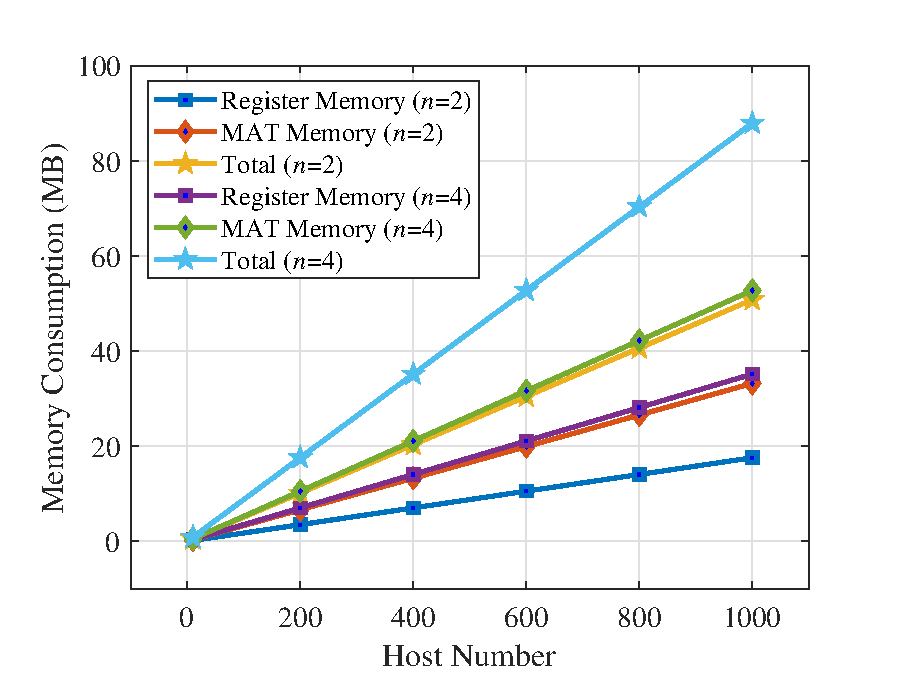
\includegraphics[scale=0.6]{figure/MemoryConsumption.eps}
            }
            \caption{Memory consumption of P4 switches.}
            \label{fig:Memory-Consumption}
            \end{figure}



\section{Security Analysis}\label{sec:security analysis}
    P4DAD is designed to mitigate DoS attacks on DAD using P4. However, P4DAD may face security threats. In this section, we demonstrate how P4DAD prevents attacks that undermine its effectiveness and availability. 

    \subsection{Attacking P4DAD-enabled Devices}
        An attacker launch attacks against the resources of P4DAD-enabled devices. For example, the attacker may attempt to send NS packets with different source addresses for duplicate detection, making the P4DAD-enabled devices create binding entries and waste memory. However, P4DAD only reserves $n$ IPv6 addresses for every port in registers. $n$ is often set as 2 or 4  in a network. According to the analysis in Section \ref{sec:scalability}, it is infeasible for the attacker to make the P4DAD-enabled devices run out of memory by launching such attacks.


    \subsection{Sharing the Same Port}
        If an attacker and legitimate users share a port of a P4DAD-enabled device by connecting a legacy switch to that port. P4DAD will create binding entries for the addresses of the attacker and legitimate users connected to the legacy switch. In such a case, the attacker can still not launch DAD DoS attacks on hosts that connect to other ports of the P4DAD-enabled device because spoofing the NDP packet will be filtered by P4DAD. However, the attacker can launch DoS attacks on DAD when the hosts connected to the same legacy switch perform duplicate address detection. Therefore, sharing the same port of a P4DAD-enabled device is not allowed, which is also claimed in Section \ref{sec:threat model}.
        

    \subsection{Privacy Considerations}
        A P4DAD-enabled device should not log information about hosts that never spoof. Besides, a P4DAD-enabled device should delete binding entries as soon as possible when the addresses are released. If the binding entries are likely to be involved in the detection, prevention, or tracing of actual target address spoofing, that information may be stored for a while, the details of which depend on the specific policy of a network.   
         


\section{Discussion}\label{sec:discussion}
    In this section, we discuss register utilization and deployment issues of P4DAD. 


    \subsection{Register Utilization}
        We explore the impact of $n$ on the register utilization of $ipv6\_reg$ and then evaluate the relationship between register memory $m_i$ and register utilization $u$. The definition of the register utilization $u$ of $ipv6\_reg$ is as follows: 
        \begin{equation}
                \label{register-utilization-calculation}
                \begin{aligned}
                    u = \frac{i}{n}\ \ (i \leq n),
                \end{aligned}
        \end{equation}
        where $i$ is the number of IPv6 addresses that a host configures to its interfaces.
        We consider three scenarios according to different address assignment mechanisms. In each scenario, a host configures a link-local address first. The details of each scenario are as follows:
        \begin{enumerate}[1)]
            \item \textbf{SLAAC-Only}: Only SLAAC is adopted. The access routers in the network periodically multicast the Router Advertisement (RA) messages \cite{NDP} to all on-link nodes with the Managed and Otherconfig flags off. RA messages contain a Prefix Information Option (PIO). When receiving RA messages, a host uses SLAAC and the prefix in PIO to configure two global unicast IPv6 addresses;

            \item \textbf{DHCPv6-Only}: Only DHCPv6 is adopted. The access routers in the network periodically multicast the RA messages to all on-link nodes with the Managed and Otherconfig flags on. When receiving this kind of RA messages, a host requests IPv6 addresses from the DHCPv6 server. The DHCPv6 server usually assigns a global unicast IPv6 address to each host;

            \item \textbf{SLAAC+DHCPv6}: Both SLAAC and DHCPv6 are adopted, and a host can configure two global unicast IPv6 addresses through SLAAC and a global unicast IPv6 address through DHCPv6.
        \end{enumerate}
        We calculate the register utilization in the above three scenarios, and the results are shown in Table \ref{tab:register-utilization}. When $n$ equals 2, a network can only adopt DHCPv6. In such a case, the register utilization reaches 100\%. When $n$ is equal to 4, a network can adopt either SLACC or DHCPv6. The register utilization reaches 100\% if hosts configure both SLAAC and DHCPv6 addresses. However, when $n$ equals 8, the register utilization decreases by half.

        \begin{table}
            \centering
            \caption{Impact of $n$ on register utilization.}
            \begin{tabular}{|c||c|c|c|}
                 \hline
                 \textbf{$n$} & \textbf{SLAAC-Only} & \textbf{DHCPv6-Only} & \textbf{SLAAC+DHCPv6} \\
                 \hline
                 \hline
                 \textbf{2} & \ding{55} & 100\% & \ding{55} \\
                 \hline
                 \textbf{4} & 75\% & 50\% & 100\% \\
                 \hline
                 \textbf{8} & 37.5\% & 25\% & 50\% \\
            \hline
            \end{tabular}
            \label{tab:register-utilization}
            \vspace{-0.3cm}
        \end{table}
        
        The register memory $m_i$ consumed by $ipv6\_reg$ is defined as follows: 
        \begin{equation}
            \label{memory-assumption-calculation}
            \begin{aligned}
                m_i = \frac{h \cdot i}{u} \cdot unit,
            \end{aligned}
        \end{equation}
        where $h$ is the number of hosts, $unit$ is the register memory size that an IPv6 address occupies, and $u$ and $i$ are shown in Equation (\ref{register-utilization-calculation}). In our example, the size of $unit$ is 15 B, with 8 B for storing an IPv6 address, 1 B for storing its state, and 6 B for storing its expiration time. As shown in Equation (\ref{memory-assumption-calculation}), under the same number of hosts and a certain number of IPv6 addresses assigned to each host, the register memory $m_i$ consumed by the switch decreases with the increase of register utilization $u$.

    \subsection{Deployment Issues}
        As P4-enabled devices may be expensive, we consider two deployment strategies for different scenarios:
        \subsubsection{First-Hop Level}
            This is an ideal deployment strategy. As shown in Fig. \ref{fig:deployment} (a), in this case, all the first-hop switches in a network are P4-enabled switches with the functionality of P4DAD, which can filter spoofed NS and NA messages. As for the aggregation level, a network can deploy legacy switches. This does not have an influence on the functionality of P4DAD.

            % \begin{figure}
            %     \centerline{
            %         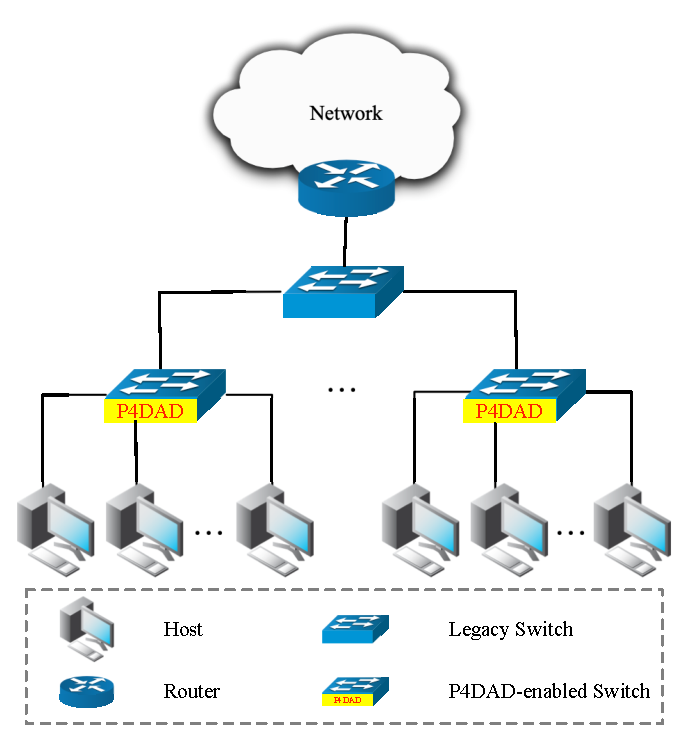
\includegraphics[scale=0.7]{figure/First-hop-deployment.eps}
            %     }
            %     \caption{First-hop level deployment.}
            %     \label{fig:first-hop deployment}
            % \end{figure}

            \begin{figure*}
                \centerline{
                    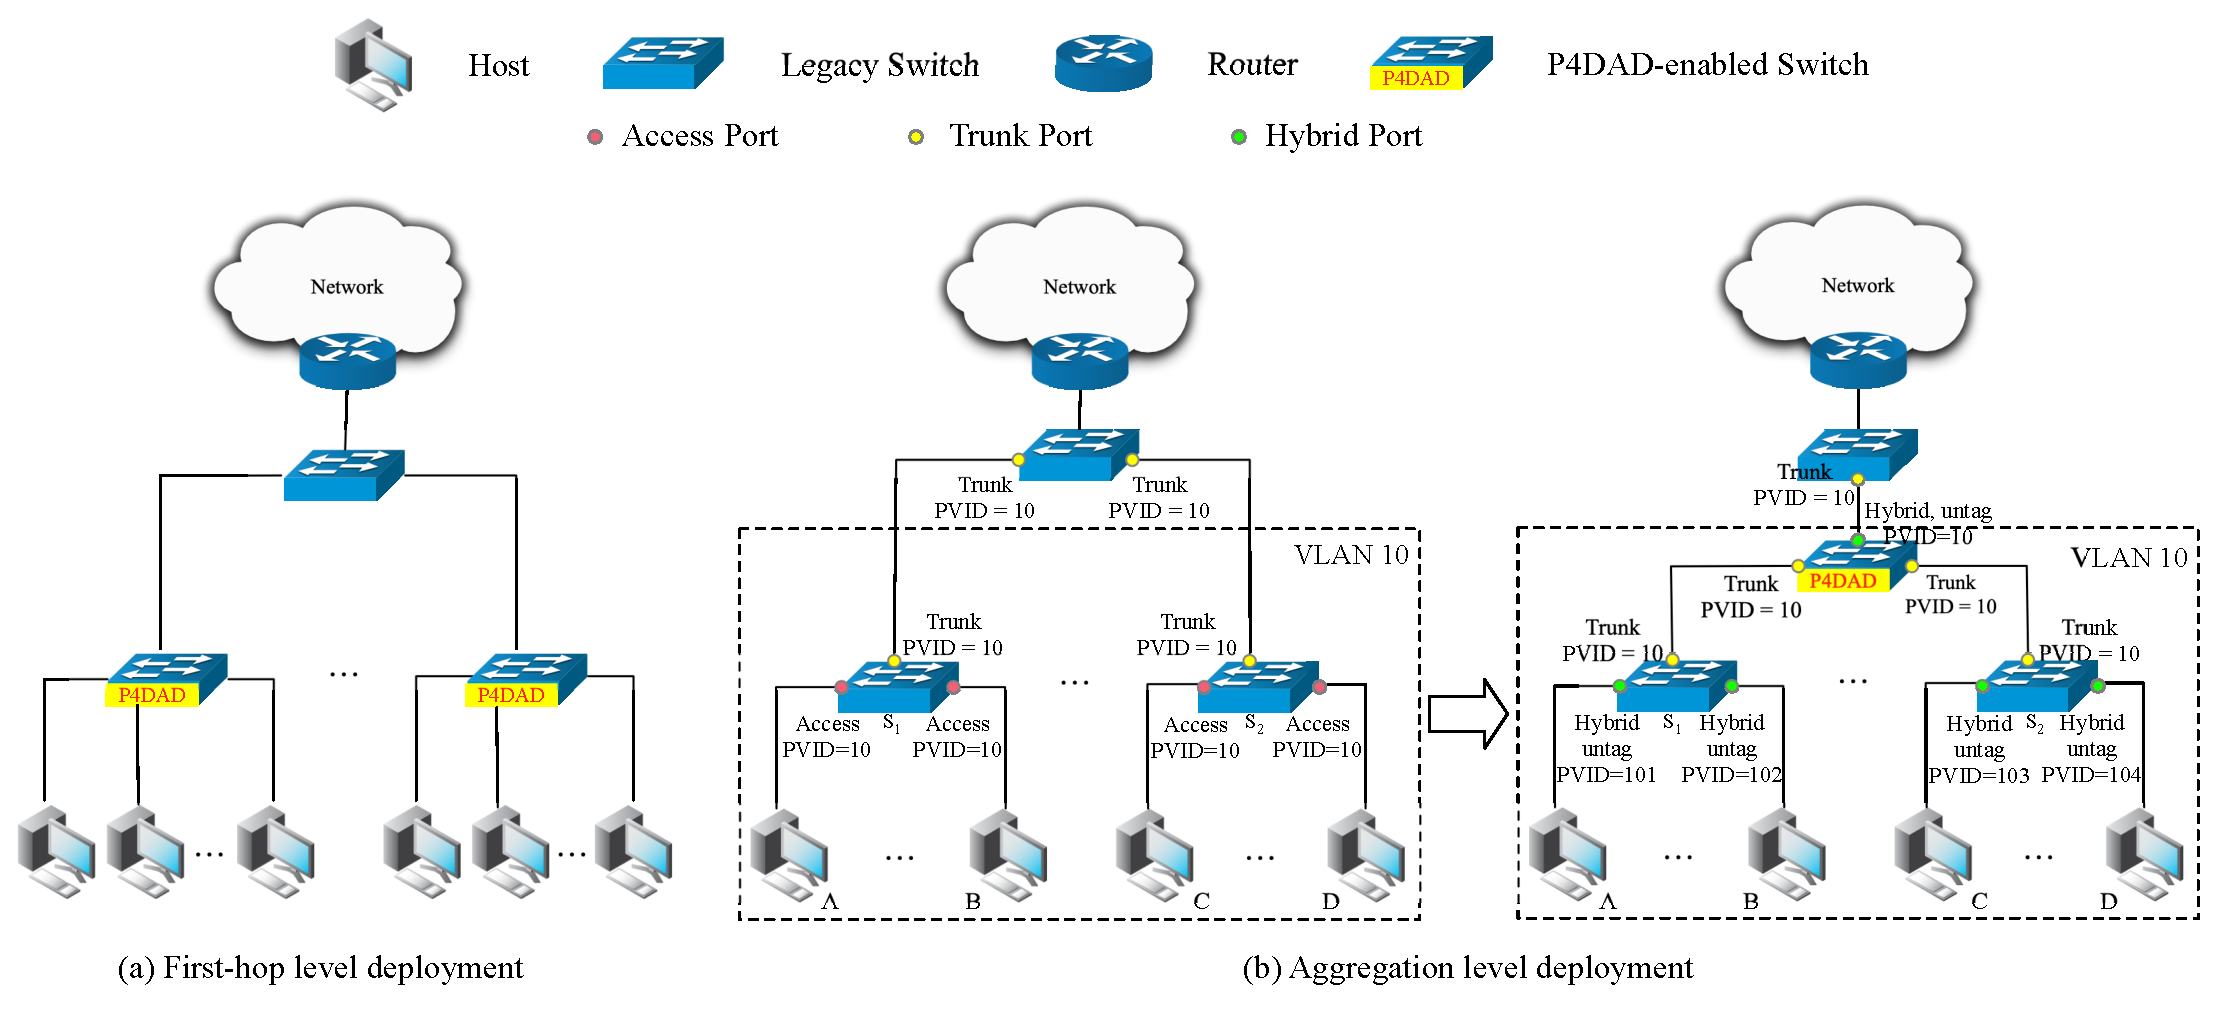
\includegraphics[scale=0.48]{figure/Deployment.eps}
                }
                \vspace{-0.2cm}
                \caption{Deployment Scenarios.}
                \label{fig:deployment}
                \vspace{-0.3cm}
            \end{figure*}

            
        \subsubsection{Aggregation Level}\label{sec:aggregation}
            % \begin{figure*}
            %     \centerline{
            %         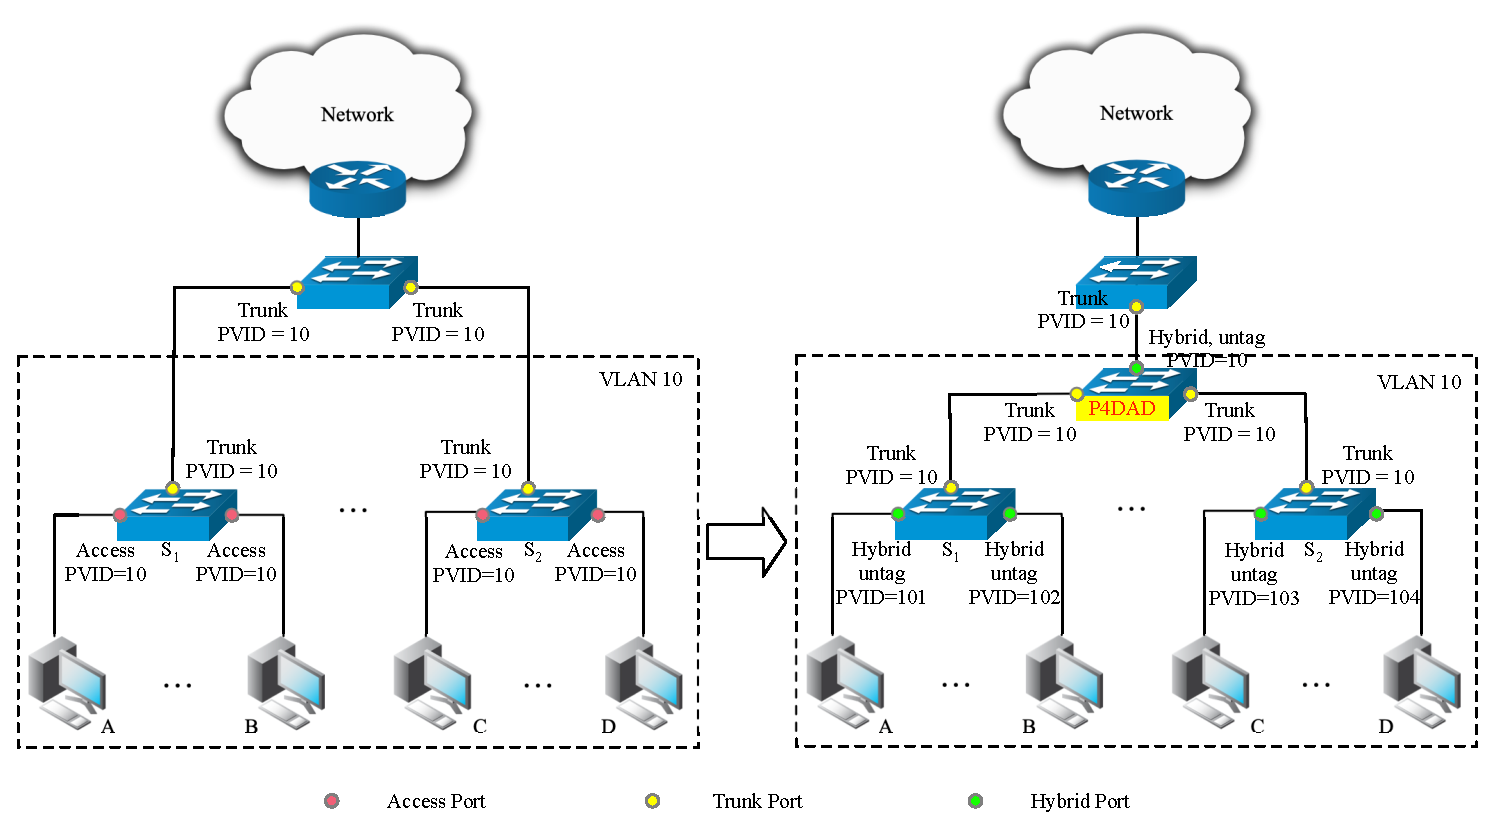
\includegraphics[scale=0.65]{figure/Aggregate-deployment.eps}
            %     }
            %     \caption{Aggregation level deployment.}
            %     \label{fig:aggregation deployment}
            % \end{figure*}
            In this scenario, we deploy a P4DAD-enabled switch for each subnet at aggregation level. The aggregation and first-hop switches do not have to be updated. A P4DAD-enabled switch is deployed between the legacy aggregation and first-hop switches. The network operator should update the configurations of each first-hop switch to help support P4DAD through virtual local area network (VLAN) classification. A deployment example is shown in Fig. \ref{fig:deployment} (b). The left sub-figure is a typical wired network topology. Generally, the number of aggregation switches are much less than that of first-hop switches. Only deploying a P4DAD-enabled switch for each subnet can save a lot of cost. In this example, there is a VLAN 10. If the network operator only deploys a P4DAD-enabled switch between the aggregation switch and first-hop switches to support P4DAD, the configurations of legacy switches should be updated as follows:
            \begin{itemize}
                \item \textbf{VLAN Classification}: All ports of the first-hop switches are configured with different VLANs (i.e., each with a unique PVID). We call them first-hop VLANs. It is assumed that the set of all the first-hop VLANs and the subnet VLANs is $P$.

                \item \textbf{Downlink Ports of First-Hop Switches}: A downlink port of a first-hop switch should be configured with a unique PVID in the subnet. The port is configured as an untagged port, and its port type is configured as \emph{hybrid}. The port allows all the VLANs from $P$ through.

                \item \textbf{Uplink Ports of First-Hop Switches}: An uplink port of a first-hop switch should be configured with the same VLAN as that of the subnet. Its port type is configured as \emph{trunk}. The port allows all the VLANs from $P$ through.

                \item \textbf{Downlink Ports of P4DAD-Enabled Switches}: A downlink port of a P4DAD-enabled switch should be configured with the same VLAN as that of the subnet. Its port type is configured as \emph{trunk}. The port allows all the VLANs from $P$ through.

                \item \textbf{Uplink Ports of P4DAD-Enabled Switches}: An uplink port of a P4DAD-enabled switch should be configured with the same VLAN as that of the subnet. Its port type is configured as \emph{hybrid}. The port allows all the VLANs from $P$ through.

                \item \textbf{Downlink Ports of Aggregation Switches}: An downlink port of an aggregation switch should be configured with the same VLAN as that of the subnet. Its port type is configured as \emph{trunk}. The port only allows subnet VLAN through.
            \end{itemize}
            
            We use a case to demonstrate the effectiveness of this strategy. Take host A as an example. We discuss the VLAN tag of its upstream and downstream traffic.
            \begin{itemize}
                \item \textbf{Upstream Traffic}: When receiving a packet from host A, switch S$_1$ will add a VLAN tag (VLAN ID = 10) in the packet according to the policy of hybrid ports. As the uplink port of switch S$_1$ allows VLAN 101 through and the VLAN tag of the packet is different from VLAN 10, S$_1$ will forward the packet according to the policy of trunk port. Similarly, the P4 switch does not change the VLAN tag when the packet arrives at its downstream port. However, when the packet leaves the uplink port of the P4 switch, the VLAN tag will be removed due to its untagged attribute. Finally, the packet will be tagged with VLAN 10 at the downlink port of the legacy aggregation switch.

                \item \textbf{Downstream Traffic}: When the legacy aggregation switch forwards a packet, it first strips the VLAN information in the packet at its downlink trunk port. The P4DAD-enabled switch adds a VLAN tag (VLAN ID = 10) in the packet at its uplink port. Similarly, when the packet is forwarded to S$_1$, it is first untagged at the downlink port of the P4DAD-enabled switch and tagged with VLAN 10 at the uplink port of S$_1$. Finally, the packet is untagged at the downlink port of S$_1$ due to its untagged attribute and forwarded to host A.
            \end{itemize}

            As we can see, a packet sent from host A will be tagged with VLAN 101 at the P4DAD-enabled switch, but with VLAN 10 at the legacy aggregation switch. VLAN 101 is transparent to the outside subnet. Under this circumstance, the P4DAD-enabled switch can use the VLAN ID as the key to store the bindings between a VLAN and IPv6 addresses and filter spoofed NS and NA messages.





\section{Conclusion}\label{sec:conclusion}
    In this paper, we propose P4DAD which is a lightweight, deployable, robust, and secure DAD mechanism. 
    By introducing P4, P4DAD secures DAD in the network without the modification of the NDP or host network stack. Also, no extra calculations are introduced to the host. By storing IPv6 addresses assigned to hosts locally and utilizing packet digests, P4DAD does not rely on a central controller and thus avoids single points of failure. 
    To the best of our knowledge, P4DAD is the first secure DAD mechanism using P4. We implement a P4DAD prototype, and our evaluation results show that P4DAD can prevent DoS attacks on DAD effectively with negligible overhead, and has satisfactory scalability. 



\section*{Acknowledgment}
    This work is supported by the National Key R\&D Program of China (Grant No. 2018YFB1800405, 2018YFB1800402, and 2017YFB0801701), and National Natural Science Foundation of China (Grant No. 61772307).

% \appendix
% \section{My Appendix}
% Appendix sections are coded under \verb+\appendix+.

% \verb+\printcredits+ command is used after appendix sections to list 
% author credit taxonomy contribution roles tagged using \verb+\credit+ 
% in frontmatter.

% \printcredits

%% Loading bibliography style file
%\bibliographystyle{model1-num-names}
\bibliographystyle{cas-model2-names}

% Loading bibliography database
% \bibliography{cas-refs}
\bibliography{ref/reference}

%\vskip3pt

\bio{}
\textbf{Lin He} is currently a postdoctoral researcher at Institute for Network Sciences and Cyberspace, Tsinghua University, China. He received his Ph.D. from Tsinghua University in 2019. His major research interests include network architecture and protocol design, Internet accountability and privacy.
\endbio

\bio{}
\textbf{Peng Kuang} is currently pursuing his master degree at Institute for Network Sciences and Cyberspace, Tsinghua University, China. His major research interests include network architecture and protocol design.
\endbio

% \bio{figs/pic1}
\bio{}
\textbf{Ying Liu} received the M.S. degree in computer science and the Ph.D. degree in applied mathematics from Xidian University, China in 1998 and 2001 respectively. She is currently an associate professor at the Tsinghua University, China. Her major research interests include network architecture design, next generation Internet architecture, routing algorithm and protocol.
\endbio

\bio{}
\textbf{Gang Ren} received the Ph.D. degree in computer system architecture from Tsinghua University, China in 2009. He is currently an associate professor at the Tsinghua University, China. His major research interests include network architecture design, next generation Internet architecture, and network security.
\endbio

\bio{}
\textbf{Jiahai Yang} received the B.S. degree from Beijing Technology and Business University, the M.S. degree and Ph.D. degree from Tsinghua University, Beijing, China; all in Computer Science. He is a professor of the Institute for Network Sciences and Cyberspace, Tsinghua University, Beijing, China. His research interests include network management, network measurement, Internet routing and applications, cloud computing and big data applications.
% He is a member of IEEE \& ACM.
\endbio

\end{document}

